\documentclass[akbc,twoside,11pt]{article}
\usepackage{akbc}
\usepackage{graphicx}
\usepackage{amsmath}
\akbcheading
\ShortHeadings{Scalable Rule Learning in Probabilistic Knowledge Bases}
{Jain, Friedman, Ku\v{z}elka, Van den Broeck, \& De Raedt}
\finalcopy % Uncomment for camera-ready version, but NOT for submission.

\usepackage{algorithm}
\usepackage[noend]{algpseudocode}

\usepackage{makecell}
\usepackage{dsfont}
\usepackage{amsfonts}
\usepackage{enumitem}
\usepackage{multirow}
\usepackage{xspace}

\setlist[enumerate]{itemsep=0mm}

\DeclareMathOperator*{\argmin}{arg\, min}
\DeclareMathOperator*{\argmax}{arg\, max}
\iffalse % Begin Block Comment 
\fi % End Block Comment
%\newtheorem{example}{Example}[section]
\newcounter{example}
\newenvironment{example}[1][]{\refstepcounter{example}\par\medskip\noindent
   \textbf{Example~\theexample #1} \rmfamily}{\medskip}
\newtheorem{definition}{Definition}

%\newcommand{\citet}[1]{\citeauthor{#1}~(\citeyear{#1})}

\newcommand{\blue}[1]{\textcolor{blue}{{#1}}}

\newcommand{\ondrej}[1]{\textcolor{red}{O: {#1}}}
\newcommand{\arcchit}[1]{\textcolor{red}{A: {#1}}}
\newcommand{\luc}[1]{\textcolor{red}{L: {#1}}}
\newcommand{\guy}[1]{\textcolor{red}{G: {#1}}}
\newcommand{\tal}[1]{\textcolor{blue}{T: {#1}}}

\newcommand{\algorithmname}{SafeLearner\xspace}

\allowdisplaybreaks

\begin{document}

\title{Scalable Rule Learning in Probabilistic Knowledge Bases}

\author{\name Arcchit Jain \email arcchit.jain@cs.kuleuven.be\\\addr KU Leuven
       \AND \name Tal Friedman \email tal@cs.ucla.edu \\\addr University of California, Los Angeles
       \AND \name Ond\v{r}ej Ku\v{z}elka \email ondrej.kuzelka@cs.kuleuven.be \\\addr KU Leuven
       \AND \name Guy Van den Broeck \email guyvdb@cs.ucla.edu \\\addr University of California, Los Angeles
       \AND \name Luc De Raedt \email luc.deraedt@cs.kuleuven.be \\\addr KU Leuven}

% For research notes, remove the comment character in the line below.
% \researchnote

\maketitle

\begin{abstract}
Knowledge Bases (KBs) are becoming increasingly large, sparse and probabilistic. These KBs are typically used to perform query inferences and rule mining. But their efficacy is only as high as their completeness. Efficiently utilizing incomplete KBs remains a major challenge as the current KB completion techniques either do not take into account the inherent uncertainty associated with each KB tuple or do not scale to large KBs.

Probabilistic rule learning not only considers the probability of every KB tuple but also tackles the problem of KB completion in an explainable way. For any given probabilistic KB, it learns probabilistic first-order rules from its relations to identify interesting patterns. But, the current probabilistic rule learning techniques perform grounding to do probabilistic inference for evaluation of candidate rules. It does not scale well to large KBs as the time complexity of inference using grounding is exponential over the size of the KB. In this paper, we present \algorithmname -- a scalable solution to probabilistic KB completion that performs probabilistic rule learning using lifted probabilistic inference -- as faster approach instead of grounding. 

We compared \algorithmname to the State-of-the-art probabilistic rule learner ProbFOIL$^+$ and to its deterministic contemporary AMIE+ on standard probabilistic KBs of NELL (Never-Ending Language Learner) and Yago. Our results demonstrate that \algorithmname scales as good as AMIE+ when learning simple rules and is also significantly faster than ProbFOIL$^+$. 
\end{abstract}


\section{Introduction}
\label{Introduction}
There is an increasing tendency to construct knowledge bases and knowledge graphs by machine learning methods. As a result, knowledge bases are often incomplete and also uncertain. To cope with uncertainty, one often resorts to probabilistic databases and logics \cite{DBLP:journals/ftdb/BroeckS17,2016Raedt}, which take into account the probability of the tuples in the querying process. The most widely used probabilistic database semantics is based on the tuple-independent probabilistic databases model, which assumes that every tuple in every table of the database is independent of one another

To cope with incomplete knowledge bases, various researchers have used machine learning techniques to learn a set of rules that can be used to infer new tuples from the existing ones, thereby completing the knowledge base \cite{NELL}. This traditional relational rule learning setting \cite{FOIL} has been extended to probabilistic logics and databases by \citet{DBLP:conf/ijcai/RaedtDTBV15}. However, the ProbFOIL approach of \citeauthor{DBLP:conf/ijcai/RaedtDTBV15} suffers from one key limitation: It does not scale well to large databases due to the grounding step, which results in an intractable probabilistic inference problem. The key contribution of this paper is the introduction of the \algorithmname system which performs two major tasks. 1) It uses lifted inference to avoid the grounding step and to improve scaling. 2) It enhances a highly efficient rule generation system, AMIE+ \cite{DBLP:journals/vldb/GalarragaTHS15} to obtain deterministic candidate rules which are then made probabilistic using lifted inference.

This paper is organized as follows. 
We introduce the background for this paper in Section~\ref{sec:back}.
We define, in Section~\ref{sec:problem}, the problem of learning a set of probabilistic rules.
Sections~\ref{sec:structure_learning} and~\ref{sec:parameter_learning} outline the idea behind the working of \algorithmname.
Section~\ref{sec:algo} proposes the algorithm for \algorithmname.
In Section~\ref{sec:exp}, we present an experimental evaluation in the context of the NELL knowledge base \cite{NELL}.
An overview of related work can be found in Section~\ref{sec:related}.
Section~\ref{sec:conc} discusses future research directions and concludes.

\section{Background}
\label{sec:back}
The notation used and definitions introduced in this section are largely adapted from the work of \citet{DBLP:conf/kr/CeylanDB16}. Throughout the paper, $\sigma$ denotes a relational vocabulary, consisting of a finite set of predicates or relations $\mathcal{R}$, and a finite set of constants or entities~$\mathcal{C}$. The \textit{Herbrand Base} of $\sigma$ is the set of all ground atoms, called $\sigma$\textit{-atoms}, of the form $R(c_1, ..., c_n)$ with $R \in {\mathcal R}$ and $c_i \in \mathcal{C}$ (that is, all tuples that can be constructed from $\mathcal{R}$ and $\mathcal{C}$). A $\sigma$-interpretation is a truth value assignment to all the $\sigma$-atoms, often represented as a set containing all the $\sigma$-atoms mapped to \textit{True}. A relational database can be seen as a $\sigma$-interpretation \cite{abiteboul1995foundations}. Here, database relations correspond to predicates and database tuples correspond to $\sigma$-atoms. The $\sigma$-atoms that are true in the $\sigma$-interpretation are those that are listed in the database tables.

\begin{table}
\begin{small}
\parbox{.48\linewidth}{
\centering
\begin{tabular}{@{}cc|c@{}}
researcher					&paper					&P\\
\hline
bob     					&plp				    &0.9\\
carl						&plp			    	&0.6\\
greg						&plp			    	&0.7\\
ian 						&db		                &0.9\\
harry						&db	                	&0.8\\
\end{tabular}
\caption{\textit{author/2}}\label{t1}
\ \\ \ \\ \ \\
\begin{tabular}{@{}cc|c@{}}
researcher					&university				&P\\
\hline
edwin						&harvard				&1.0\\
fred						&harvard				&0.9\\
alice						&mit					&0.6\\
dave						&mit					&0.7\\
\end{tabular}
\caption{\textit{location/2}}\label{t2}
}
\hfill
\parbox{.48\linewidth}{
\centering
\begin{tabular}{@{}cc|c@{}}
researcher					&researcher				&P\\
\hline
alice						&edwin			    	&0.2\\
alice						&fred					&0.3\\
bob					        &carl					&0.4\\
bob					        &greg					&0.5\\
bob					        &harry					&0.6\\
bob					        &ian			    	&0.7\\
carl						&greg					&0.8\\
carl						&harry					&0.9\\
carl						&ian			    	&0.8\\
dave						&edwin		    		&0.7\\
dave						&fred					&0.6\\
edwin						&fred					&0.5\\
greg						&harry					&0.4\\
greg						&ian		    		&0.3\\
ian						    &ian	    			&0.2\\
\end{tabular}
\caption{\textit{coauthor/2}}\label{t3}
}
\end{small}\label{coauthor_example}
\end{table}


\subsection{Queries} \label{queries}

In databases (represented as $\sigma$-interpretations), query answering can be formalized as follows. A query is a first-order logic formula $Q(x_1,x_2,\dots, x_k)$ with free variables $x_1$, $x_2$, $\dots$, $x_k$. The task of answering the query translates to finding the set of all substitutions $[x_1/t_1,$ $x_2/t_2,$ $\dots,$ $x_k/t_k]$ such that $\omega \models Q[x_1/t_1,x_2/t_2,\dots,x_k/t_k]$. The answer to a query $Q$ w.r.t. a database $\omega$ is denoted as $\operatorname{Ans}(Q,\omega)$.

\begin{example}\label{ex:query_answering}
Consider the database consisting of Tables \ref{t1}, \ref{t2} and \ref{t3} and the query 
$Q_1(x) = \mathsf{location}(x, \mathsf{mit}) \wedge \mathsf{coauthor}(x, \mathsf{fred})$. Then the answer to the query $Q$ consists of the following substitutions: $[x/\mathsf{alice}]$ and $[x/\mathsf{dave}]$. In general, queries may also contain variables bound by existential or universal quantifiers. For instance, if we have the query
$Q_2(z) = \exists x, y .\; \mathsf{location}(z, x) \wedge \mathsf{coauthor}(z, y) $, which asks for researchers from the database that are located at some university and are coauthors with someone, then the answer consists of the substitutions $[z/\mathsf{edwin}]$, $[z/\mathsf{alice}]$ and $[z/\mathsf{dave}]$.
\end{example}

A {\em Boolean query} is a query with fully quantified variables. A {\em conjunctive query} (CQ) is a negation-free first-order logic conjunction with all variables either free or bound by an existential quantifier. A {\em union of conjunctive queries} (UCQ) is a disjunction of conjunctive queries. We mainly work with UCQs in this paper. 

Conjunctive queries may also be expressed using Prolog notation \cite{DBLP:books/sp/ClocksinM81}. For instance, the rule $\mathsf{R}(z) \mbox{ :--}\; \mathsf{location}(z,x), \mathsf{coauthor}(z,y).$ represents the query $Q_2$ from Example \ref{ex:query_answering}. 
 Here, $\mathsf{R}(z)$ is called {\em head} of the rule\footnote{The choice for the relation $\mathsf{R}$ ($\notin \mathcal{R}$) was arbitrary here.} and $\mathsf{location}(z,x), \mathsf{coauthor}(z,y)$ is called the {\em body}. The rule is understood as defining tuples of a new table $\mathsf{R}$ that, in this case, contains all tuples $[t]$ where $[z/t] \in \operatorname{Ans}(\exists x, y.\; \mathsf{location}(z,x) \wedge \mathsf{coauthor}(z,y), \omega)$. Thus, variables not occurring in the head of the rule correspond to existentially quantified variables in the respective conjunctive query. In Prolog notation, UCQs are represented as a collection of rules with the same relation in the head. For a given set of rules representing a UCQ, we denote {\em prediction set} as the union of its respective answer sets.


\subsection{Probabilistic Databases (PDBs)} 

A database $\mathcal{D}$ is said to be a PDB if its every tuple has an assigned probability value. Mathematically, A PDB $\mathcal{D}$, for a vocabulary $\sigma$, is a finite set of tuples of the form $\langle t, p \rangle$, where $t$ is a $\sigma$-atom and $p \in [0,1]$. Moreover, if $\langle t, p \rangle \in \mathcal{D}$ and $\langle t, q \rangle \in \mathcal{D}$, then $p = q$. Each PDB for the vocabulary $\sigma$ induces a unique probability distribution over $\sigma$-interpretations~$\omega$:
\begin{equation}
\mathrm{P}_\mathcal{D}(\omega) = \prod_{t \in \omega} \mathrm{P}_\mathcal{D}(t)\prod_{t \notin \omega} (1 - \mathrm{P}_\mathcal{D}(t)),
\end{equation}
where
\begin{equation*}\mathrm{P}_\mathcal{D}(t) = \begin{cases} 
p & \mbox{if }  \langle t, p \rangle \in \mathcal{D} \\
0 & \mbox{otherwise.}
\end{cases}
\end{equation*}

\begin{example}\label{coauthor_example} Tables \ref{t1}, \ref{t2} and \ref{t3} form a PDB with 3 relations: $\mathsf{coauthor/2}$, $\mathsf{author/2}$ and $\mathsf{location/2}$.
\end{example}

%Choosing $\mathrm{P}_\mathcal{D}(t) = 0$ for tuples missing from PDB $\mathcal{D}$ is the probabilistic version of the CWA. 
Furthermore, the probability of any Boolean query $Q$ w.r.t. a PDB $\mathcal{D}$ is
\begin{equation}\label{eq:def_query_probability}
\mathrm{P}_\mathcal{D}(Q) = \sum_{\omega \models Q} \mathrm{P}_\mathcal{D}(\omega).
\end{equation}

\begin{example}
For the Boolean query
$Q_3 = \mathsf{coauthor}(\mathsf{bob}, \mathsf{carl})$
we can read off the probability $\mathrm{P}_\mathcal{D}(Q_3) = 0.4$ directly from Table \ref{t3}. On the other hand, the probability of query
$Q_4 = \exists x.\; \mathsf{coauthor}(\mathsf{bob}, x) \wedge$ $\mathsf{coauthor}(\mathsf{carl}, x)$
cannot be read directly from any table and requires probabilistic inference.  Directly using Equation~\ref{eq:def_query_probability}, we get $\mathrm{P}_\mathcal{D}(Q_4) = 0.879 $. Intuitively, $Q_3$ asked about the probability that $\mathsf{bob}$ and $\mathsf{carl}$ are co-authors, whereas $Q_4$ asked about the probability that $\mathsf{bob}$ and $\mathsf{carl}$ have a common co-author.
\end{example}


% \subsection{$\lambda$-completion of PDBs} 

% Consider a PDB $\mathcal{D}$. The tuples which can be constructed from the already existing constants in $\mathcal{C}$ but do not lie in a given PDB $\mathcal{D}$ are called \textit{open-world tuples} w.r.t. $\mathcal{D}$. Let $\lambda: \mathcal{R} \to [0,1]$ be a function we will call the {\em $\lambda$-parameter} which, for any relation $r$, denotes the probability assigned to any open-world tuple of $\mathsf{r}$. A $\lambda$\textit{-completion} of a PDB $\mathcal{D}$ is then defined as another PDB $\mathcal{D}_\lambda = \mathcal{D}\ \cup\ \{ \langle t, \lambda(\operatorname{rel}(t)) \rangle\ |\ \neg \exists q, \langle t, q \rangle \in \mathcal{D}\}$ where $\operatorname{rel}(t)$ denotes the relation of the $\sigma$-atom~\textit{t}. PDB $\mathcal{D}_\lambda$ can be thought of as an extension of $\mathcal{D}$ where all the open-world $\sigma$\textit{-atoms} of relation $r$ exist with  probability $\lambda(r)$. For any Boolean query $Q$ and a $\lambda$-completion $\mathcal{D}_\lambda$, the probability of the query is
% \begin{equation*}
% \mathrm{P}_{\mathcal{D}_\lambda}(Q) = \sum_{\omega \models Q} \left( \prod_{t \in \omega} \mathrm{P}_\mathcal{D}(t)\prod_{t \notin \omega} \Big(1 - \mathrm{P}_{\mathcal{D}_\lambda}(t)\Big)\right)
% \end{equation*}
% \begin{equation*}
% \mathrm{P}_{\mathcal{D}_\lambda}(t) = \begin{cases} 
% p & \mbox{if } \exists\ p \mbox{ such that } \langle t, p \rangle \in \mathcal{D} \\
% \lambda(\operatorname{rel}(t)) & \mbox{otherwise} \\
% \end{cases}
% \end{equation*}
% \citet{DBLP:conf/kr/CeylanDB16} provide a detailed discussion of the resulting open-world semantics for probabilistic databases, and they provide several arguments and examples why this setting is more natural for many applications, such as those involving knowledge graphs.


% \subsection{Query Plans} 

%  A query plan is a sequence of database operations (namely join, projection, union, selection and difference) that are executed to do exact probabilistic inference for a query \cite{DBLP:journals/ftdb/BroeckS17}. %\ondrej{It is not clear from this description how exact probabilistic inference is performed because you have not defined the probabilitic variants of these queries - called ``extensional operators'' in the survey of Guy and Dan Suciu.}. \arcchit{I can't explain that in the span of 15 page limit of the paper, so I have cited them}
%  Extensional query plans are query plans under an added tuple-independent assumption - the assumption that every tuple in every table of the database is independent of one another. Query plans are useful because query inference can be done by first constructing a query plan and then executing it to get the query probability. In general, for every UCQ, the complexity of evaluating it on a probabilistic database is either PTIME or \#P-complete in the size of the database~\cite{dalvi2012dichotomy}. Those UCQs for which a correct extensional query plan exist and so these get evaluated in polynomial time are referred to as Safe Queries. 


% \subsection{Lifted Inference} 

% \ondrej{remove references to OW lifted inference}
% In this paper, we exploit lifted inference algorithm $\textit{Lift}^R_O$ \cite{DBLP:conf/kr/CeylanDB16} for probabilistic inference. This algorithm is an extension of the $\textit{Lift}^R$ algorithm \cite{DBLP:conf/uai/GribkoffBS14} to the open-world probabilistic databases setting. In summary, $\textit{Lift}_O^R$ can compute the probability $\mathrm{P}_{\mathcal{D}_\lambda}(Q)$ in polynomial-time data complexity for all efficient monotone safe UCQs \cite{DBLP:conf/kr/CeylanDB16}. The $Lift^O_R$ algorithm, which is implemented in SafeSample package \cite{SafeSample}, inputs $\lambda$ and a UCQ (pertaining to the hypothesis instantiated for an example). It has 2 major steps. Firstly, it tries to decompose the query into simpler queries and thus generate a safe query plan. Secondly, it executes the safe query plan to get the probability of the query. This divide and conquer approach, to calculate the open-world probability of the query as an expression in terms of $\lambda$. Although, lifted inference can only be applied to safe queries, it is faster and more tractable than conventional probabilistic inference approaches \cite{DBLP:journals/ftdb/BroeckS17}.
% %that use grounding.\ondrej{Do we even need to refer to grounding here?}

\subsection{Lifted Inference}

A query plan is a sequence of database operations (namely join, projection, union, selection and difference) that are executed to do exact probabilistic inference for a query \cite{DBLP:journals/ftdb/BroeckS17}. %\ondrej{It is not clear from this description how exact probabilistic inference is performed because you have not defined the probabilitic variants of these queries - called ``extensional operators'' in the survey of Guy and Dan Suciu.}. \arcchit{I can't explain that in the span of 15 page limit of the paper, so I have cited them}
Extensional query plans are query plans under the tuple-independence assumption. Extensional query plans can be used to compute probabilities of queries over probabilistic databases. However, not all queries have an extensional query plan that can be used to compute their probabilities correctly. Those for which such a correct extensional query plan exists are called {\em safe queries}. Hence, safe queries can be evaluated in time polynomial in the size of the database (data complexity). In general, for every UCQ, the complexity of evaluating it on a probabilistic database is either PTIME (safe queries) or \#P-complete in the size of the database~\cite{dalvi2012dichotomy}. The algorithms with PTIME data complexity are also called {\em lifted inference algorithms}. In this work, we exploit the lifted inference algorithm of $Lift^O_R$ which is an extension of the $\textit{Lift}^R$ algorithm \cite{DBLP:conf/uai/GribkoffBS14}. The $Lift^O_R$ algorithm exploits the structure of a query and uses a divide and conquer approach to calculate its probability.  

%Query plans are useful because query inference can be done by first constructing a query plan and then executing it to get the query probability. In general, for every UCQ, the complexity of evaluating it on a probabilistic database is either PTIME or \#P-complete in the size of the database~\cite{dalvi2012dichotomy}. Those UCQs for which a correct extensional query plan exist and so these get evaluated in polynomial time are referred to as Safe Queries.

\subsection{Probabilistic Rules} \label{sub:probrules}%First order rules with the structure: $p\ ::\ head :- body.$ \\ where $p$ is the probability value with which the $head$ is true when the $body$ is true, $head$ is $target(A,B)$ (if its arity is 2) in this case and $body$ is a conjunction of ungrounded and positive atoms constructed with any relation in the PDB $D$.


When we have a probabilistic database and a collection of Prolog rules defining a relation $R$, the relation $R$ becomes a random variable.\footnote{Here we use the term ``random variable'' in a broad sense; similarly as we may have matrix-valued random variables, we may also have random variables that represent database relations.} The relation $R$ does no longer have to be representable as a tuple-independent table, though. Additionally, one may enlarge the set of probability distributions over tuples of $R$ that can be modelled by Prolog rules by introducing auxiliary probabilistic tables, not originally present in the database and using them in the rules. In this way, one can think of Prolog rules as a model of a distribution rather than only as a way to query a pre-existing probabilistic database. This is illustrated by the next example.

\begin{example}
As an example, let us consider again the database that is listed in Tables \ref{t1}, \ref{t2} and \ref{t3} and a rule $R(x,y) \mbox{ \textnormal{:--}}\; \mathsf{coauthor}(x,y)$. Suppose that we introduce a new probabilistic relation $\mathsf{A}(x,y)$ with all possible $\sigma$-atoms $\mathsf{A}(t_1,t_2)$ having the same probability $p$ and replace the original rule by $R(x,y) \mbox{ \textnormal{:--}}\; \mathsf{coauthor}(x,y), \mathsf{A}(x,y)$. By changing the parameter $p$ we can now decrease the probabilities of the $\sigma$-atoms $R(t_1,t_2)$. 
\end{example}

We use the following notation as syntactic sugar for probabilistic rules. We write $p :: R(x,y) \mbox{ \textnormal{:--}}\; \mathsf{coauthor}(x,y)$ to denote $R(x,y) \mbox{ \textnormal{:--}}\; \mathsf{coauthor}(x,y), \mathsf{A}_{R,i}(x,y)$ where we set $P_{\mathcal{D}}[\mathsf{A}_{R,i}(t_1,t_2)] = p$ for all tuples $(t_1, t_2)$ and where $i$ is an identifier of the respective rule. 
%\ondrej{need to rewrite this: } This can be efficiently emulated by setting the open-world probability $\lambda(\mathsf{A}_{R,i}) = p$ without actually having to explicitly enumerate tuples in the database. 
For rules with variables appearing in the body but not in the head, such as $p :: R(x,y) \mbox{ \textnormal{:--}}\; \mathsf{author}(x,z), \mathsf{author}(y,z)$, the auxiliary relation's arguments range only over the variables in the head; that is for the considered rule we would have $R(x,y) \mbox{ \textnormal{:--}}\; \mathsf{author}(x,z),$ $\mathsf{author}(y,z),$ $\mathsf{A}_{R,i}(x,y).$ 
This restriction is necessary in order to keep the resulting rules simple enough so that lifted inference could still be used, i.e.\ we want to avoid the introduction of rule's probabilistic weights to result in creating unsafe queries from safe ones. Moreover, since we will only be querying probability of individual (ground) tuples, it will be possible to create the relation $\mathsf{A}_{R,i}(x,y)$ always on the fly to contain just one tuple.

As mentioned above, relations defined using probabilistic rules do not have to be tuple-independent. Since the main intended application of the present work is to be able to fill in missing probabilistic tuples into tuple-independent probabilistic databases, we introduce the following operation, denoted $\operatorname{Ind}(R)$, which produces a tuple-independent relation $R'$ from a given relation $R$ by simply assigning marginal probabilities to the individual tuples. We may notice that when $R$ is defined using probabilistic rules and deterministic relations, i.e. relations where every tuple has probability either $0$ or $1$, then $R = \operatorname{Ind}(R)$. This can also be seen as {materializing views to tuple-independent tables.}


% \subsection{Prediction set of a rule} 

% A first-order rule could be instantiated by substituting all the free variables with constants from $\mathcal{C}$. The head of an instantiated rule is called a \textit{prediction}, if all the $\sigma$-atoms in the rule's body appear in $\mathcal{D}$. Consequently, a \textit{prediction set} for a rule is a set of all the predictions of the rule.
% \begin{example}
% Let us consider the following rule: $0.7 :: \mathsf{coauthor}(x,y) \mbox{ \textnormal{:--}}\; \mathsf{author}(x,z), \mathsf{author}(y,z).$ Here, $\mathsf{author}(\mathsf{ian}, \mathsf{db})$ is a prediction of this rule since $\mathsf{coauthor}(\mathsf{ian}, \mathsf{harry})$ and $\mathsf{author}(\mathsf{harry}, \mathsf{db})$ lie in the PDB. We need not consider its probability in the calculation of prediction set. As long as it is non-zero, there is a non-zero possibility of each of these tuples getting predicted by this rule.
% \end{example}

\section{Problem Specification}
\label{sec:problem}
We aim to learn probabilistic rules from a given PDB $\mathcal{D}$ and a target relation, $target$. We call $E$ the set of the tuples, of $target$, present in  $\mathcal{D}$. We could interpret the set of these probabilistic training examples $E$ as defining a distribution over deterministic training sets in the same way as a probabilistic database represents a distribution over deterministic databases. Then, given a probabilistic database, during training we search for a collection of probabilistic rules so that we would obtain a {\it good} model for the data. 

\begin{example}
Consider a set of examples for a relation $\mathsf{supervisor}$: $E = \{ \langle [\mathsf{greg}, \mathsf{carl}], 0.8 \rangle,\\ \langle [\mathsf{edwin}, \mathsf{fred}], 0.4 \rangle \}$ for the database from Tables \ref{t1}, \ref{t2}, \ref{t3}. The task is then to find rules that define the relation $\mathsf{supervisor}$ using the relations $\mathsf{author}$, $\mathsf{location}$ and $\mathsf{coauthor}$. For instance, one such, not particularly optimal, model could be $0.1 :: \mathsf{supervisor}(x,y) \mbox{ \textnormal{:--}}\; \mathsf{coauthor}(x,y)$.
\end{example}

What we will call a {\it good} model, depends on the context (in the next section, we consider different loss functions which could lead to different ways to score the learned probabilistic models). Moreover, what is deemed a {\it good} model also depends on the assumptions about the way the training tuples were obtained and on what we assume about the tuples that are not present in the set of training examples. We now describe the problem Statement formally as follows.

\paragraph{Given:} PDB $\mathcal{D}$, a target relation $target$, and loss function $\mathcal{L}$.
% \begin{enumerate}
%     \item PDB $\mathcal{D}$
%     \item A target relation, $target$
%     \item Loss function, $\mathcal{L}$ %(optional)\ondrej{not just optional}
%     %\item Type constraints for each relation in $\mathcal{D}$ (optional)\ondrej{I would not talk about that now}
% \end{enumerate}

\paragraph{Find:}
A set of probabilistic rules called $H = \{h_1, h_2, \ldots, h_n\}$ with $target$ in the head of each rule such that $\mathcal{L}(H)$ is minimum over all the $target$ tuples w.r.t. $\mathcal{D}$.\\

\noindent \algorithmname addresses the above Stated problem heuristically using two main components. 1) A structure learning component that generates candidate rules --- a larger set of rules that subsumes $H$. 2) A parameter learning component that optimizes weights of these rules thus effectively also performing selection of these rules as a result. We present each of these components in Sections~\ref{sec:structure_learning} and~\ref{sec:parameter_learning} respectively before explaining the algorithm of \algorithmname in Section~\ref{sec:algo}. 

\section{Structure Learning}
\label{sec:structure_learning}
Most relations of KBs have binary relations and we restrict ourselves to it. In order to learn structure in this specified problem setting, we learn deterministic candidate rules. %\ondrej{that's not true in general but we do it that way, indeed - try rephrasing. Also not clear here what ``candidate rules'' are.} 
This method of structure learning without considering the parameters $p_h$ is simpler than the case when the structure and parameters are learned jointly. But this method is followed keeping in mind that the parameters are tuned later. 
%\ondrej{Here, it is not completely clear what ``simpler method'' really refers to}, 
We use AMIE+ for generating candidate rules. It is a highly efficient rule generation system for mining deterministic rules from KBs. It uses a language bias (constraints on the form of mined rules) to mine the rules from a vast search space. Compared with a naive support-based confidence score \cite{DBLP:conf/sigmod/AgrawalIS93}, it uses a more involved scoring function. %which also takes into account the open-world nature of the data. %\ondrej{cite some association rule mining for ``confidence score''}
%\ondrej{maybe give it a name or say that you will call it confidence anyway in the rest of the paper}
By \textit{confidence}, we refer to the confidence score used by AMIE+, throughout the rest of the paper. A rule is output when it satisfies some properties \citep{DBLP:journals/vldb/GalarragaTHS15}, its confidence score surpasses a specified confidence threshold, and improves over the confidence scores of all its parents.

%\subsection{Properties of rules generated by AMIE+}
%As explained in detail by \citet{DBLP:journals/vldb/GalarragaTHS15}, there are three major properties of the rules generated by AMIE+. First, the rules are connected, i.e., there is no atom in either the head or body of the rules that does not share any of its variables with any other atom in the same rule. In other words, AMIE+ restricts generating disconnected rules like $\mathsf{supervisor}(a,b) \mbox{ \textnormal{:--}}\; \mathsf{coauthor}(c,d)$. Second, the rules are always closed, i.e., there is no atom in the head or body of the rules that has a variable unique to that atom. Thus, no variable in a rule can only appear just once. Third, the rules cannot have a reflexive atom of the form $\mathsf{R}(x,x)$.\ondrej{I am not completely convinced about this paragraph and its importance. It is indeed useful to have types for 2 reasons: (i) it probably speeds up AMIE and (ii) we need to know it for OWA learning (because the domain sizes depend on that).} \arcchit{Luc asked to explain the working of AMIE+ as it is an important part of \algorithmname. I could also comment this paragraph and just say all the rules mined by AMIE+ are independent of each other.}

% \subsection{Enforcing type constraints}
% Besides the restriction on rules by AMIE+, the structure of the model could depend on the given type constraints of few or all of the relations in $\mathcal{D}$. The information about the domain and range of each relation is often also available with the KB. Whenever provided, such information, which is not used in AMIE+, could always help the model in learning better and more relevant rules. Type constraints could restrict our model to learn only reasonable rules, as demonstrated by the next example.

% \begin{example}
% For the PDB from Tables \ref{t1}, \ref{t2}, \ref{t3}, the following type-constraints could be defined: $\{\mathsf{author}(\mathsf{researcher}, \mathsf{paper}), \mathsf{location}(\mathsf{researcher}, \mathsf{university}), \mathsf{coauthor}(\mathsf{researcher}, \mathsf{researcher})\}$. \\The enforcement of these type constraints would prevent the model to learn absurd rules like $0.1 :: \mathsf{coauthor}(x,y) \mbox{ \textnormal{:--}}\; \mathsf{author}(x,y)$ where $y$ can either be of type $researcher$ or $paper$, resulting in a contradiction. 
% \end{example} 

\subsection{Generating Candidate Rules} \label{sub:crg} Since AMIE+ expects deterministic input, we have to first generate a deterministic database from the given probabilistic database and the given training set. This may be achieved either directly by sampling from the database or by keeping only tuples that have probabilities over some threshold. The rationale behind this simple approach is as follows. Let us suppose that the training data was generated by directly sampling from a model consisting of a probabilistic database together with some probabilistic rules. Suppose that the rules contained the rule $0.7 :: \mathsf{author}(a,p) \mbox{ :--}\; \mathsf{author}(b,p), \mathsf{supervisor}(a,b)$. We may then reasonably expect that a deterministic rule learner, such as AMIE+, will be able to find the respective deterministic rule since its confidence should be on average at least $0.7$ on datasets sampled form the data-generating model. At least on a heuristic level, this justifies using a deterministic rule learner for finding candidate rules. Ideally, this intermediate deterministic step wanes the predictive performance in comparison to the case where candidates could be obtained on the probabilistic tuples \cite{DBLP:conf/ijcai/RaedtDTBV15} but this slight decrease in performance is compensated by the improvement in the scalability provided by AMIE+. Unless specified otherwise by the user, \algorithmname uses AMIE+ restricted to rules with two atoms in the body.
Then, the algorithm selects $k$ rules with highest confidence as the candidates, where $k$ is a parameter of the algorithm, and checks if the resulting rule set correspond to a safe UCQ. If the UCQ is not safe, it removes the minimal number of lowest-confidence candidate rules that make the resulting UCQ safe. Finally, we add a rule for the $target$ relation that has an empty body. Whenever this rule has non-zero probabilistic weight, all the possible tuples will have non-zero probability (this turns out to be important for avoiding infinite cross entropy scores).

\section{Parameter Learning}
\label{sec:parameter_learning}

% In this section, we discuss several approaches to learning parameters of probabilistic rule sets from PDBs.

% \subsection{Parameter Learning as Likelihood Maximization}

% \ondrej{Except there is the problem that, strictly speaking, we have just one sample from relational data. Hence, we need the additional independence assumptions, which is why I thought it needed a bit more explanation and why it was and still is a bit too long.}

Since we are learning a distribution over databases, the natural choice is to measure the likelihood of the model consisting of the learned rules given the training data. However, our training datasets are also probabilistic themselves. Thus, we need to measure how `close' the learned distributions are to the distributions of the training data. This is typically measured by the KL divergence. Another way to look at this problem is by asking what the likelihood would be given the data sampled from the training distribution. This is an expectation of likelihood, or cross entropy, which turns out, is equivalent to KL divergence (up to a constant) when we assume both independence of the tuples and independence of the predictions (i.e. we replace the target relation $R$ by its materialization $R' = \operatorname{Ind}(R)$).
%One way to learn probabilistic models is to maximize likelihood of the model given the training data. The training examples are probabilistic, so, as we will see, under the independent tuple assumption, maximizing the likelihood will correspond to minimization of cross entropy. 
%Let us briefly discuss why this is the case. 
This can be seen as follows. First, let us assume that the training examples are complete, that is, the training set $E$ contains all possible tuples $t_i$ and their respective probabilities $p_i$. %Furthermore, assume that a set of probabilistic rules is given and that we want to determine their parameters by optimizing the expected log-likelihood.
%We assume that the training examples (tuples) are independent, i.e. that they are no different than any other relation defined in the probabilistic database. It turns out that we also need to assume that the predictions can be represented as a tuple-independent relation $R'$ as well, i.e.\ we work with the materialization $R' = \operatorname{Ind}(R)$ of the target relation $R$. 
Then, we can write the expected log-likelihood of the model given the training examples as follows. Let $\mathbf{T}$ be the set of all possible tuples. For every $i \in \{1,\dots,|\mathbf{T}|\}$, let $T_i$ be a Bernoulli random variable corresponding to the $i$-th training example $\langle t_i, p_i \rangle \in E$ such that $P[T_i = 1] = p_i$. Next let $q_i$ denote the probability assigned by the model to the tuple $t_i$. Then we may write the expected log-likelihood as 
\begin{equation}
    \mathbb{E}\left[ \log{\left( \prod_{ t_i \in \mathbf{T}} q_i^{\mathds{1}(T_i = 1)} \cdot (1-q_i)^{\mathds{1}(T_i = 0)} \right)} \right]
    = \sum_{\langle t_i, p_i \rangle \in E} \left( p_i \log{ q_i} + (1-p_i) \log{\left( 1-q_i \right)} \right)
\end{equation}
where the expectation is over the samples of the probabilistic database (here represented by the variables $T_i$).
%\guy{There are some issues with the notation in the equation above. It would be better to say what the expectation is over. And the fact the $p_i$ and $E$ appear inside of the expectation is a little confusing, since they are in fact what defines the expectation on the outside.}
This is the same as cross entropy, except for the sign. Hence, what we need to minimize is indeed cross entropy.
%\guy{I still think it's more natural to say: let's assume that both data and predictions are tuple-independent tables, and compute the KL divergence between them. Isn't this more natural than expected likelihood?} - ok, I changed based on your first suggestion above

%Obviously it is unrealistic to expect that we would have a complete set of training examples.

\subsection{Estimating Losses from Incomplete Training Data}

Naturally, in most realistic cases, access to probabilities of all the possible tuples is limited. We introduce two distinct settings that lead to a different way of treating tuples that are outside the training set.  % \ondrej{I started adding something more here, to also have a setting a bit closer to original ProbFOIL besides the more SRL setting that we have described so far}

\subsubsection{Learning Models for the Whole Database}\label{sub:samp}

In the first setting, we assume that our goal is to learn a probabilistic model for the whole database. Since most domains will be sparse, we may assume that a majority of the tuples (over elements of the given domain) will have some very small probability $\gamma_{\textit{target}}$, possibly zero. %, paralleling the assumptions from the open world databases semantics that we use in this paper. 
When estimating the loss of a set of rules $Q$ (here represented as a UCQ), we need to split the possible $target$ tuples (Cartesian product of sets of constants of all the entities constituting the $target$) into three categories: 
\begin{enumerate}
    \item $target$ tuples contained in the training set, also denoted by the set of examples $E$.
    \item possible $target$ tuples outside $E$ that lie in the answer of $Q'$ (i.e. in $\operatorname{Ans}(Q')$), where $Q'$ contains all the rules in $Q$ with non-empty bodies. These are all the $target$ tuples outside $E$ that have at least one grounded proof in the training data. In other words, these tuples can be inferred from the training data by the rules in $Q'$.
    \item the remaining possible $target$ tuples. These tuples are neither present in the training data nor can these be inferred from the training data by the rules in $Q'$.
\end{enumerate}
%{\color{red} Earlier text: (i) $target$ tuples contained in the training set, (ii) target tuples outside the training set that are contained in the answer of $Q'$ (i.e. in $\operatorname{Ans}(Q')$), where $Q'$ is the same as $Q$ but without the rule with empty body, and (iii) the other possible target tuples.} 
The estimate of the loss is then obtained as the sum of estimates of these three losses. Estimating the first and second component of the loss is straightforward. To speed it up, we estimate the second component only on a sample of the tuples of the second category (as there may often be significantly more tuples in this category than in the first one).
%The tuples in the third category are irrelevant for weight learning, because no matter how we set, and we can ignore them.\ondrej{something weird here - we do use the rule with body = true, right? so this is }
Similarly, it is not difficult to estimate the third component of the loss because it only depends on the probability of the rule with empty body and all tuples in this third category have the same estimated probability.

We will denote by $E$, $E_2$, $E_3$ the sets of sampled tuples for categories 1, 2 and 3, respectively.
The weights of tuples in $E_2$ and $E_3$ are calculated corresponding to the inverse of the subsampling ratio. For example, if we sample 5000 tuples out of a possible set of 100000, we assign a weight of 20 to each of the sampled tuples. Tuples in $E_2$ are assigned a weight $w_2$ and tuples in $E_3$ are assigned $w_3$. %These are defined as follows:
% \begin{equation*}
% \begin{aligned}
% w_1 &= \frac{\mbox{$\mid (\cup_i$ Prediction set of $h_i) \setminus E \mid$}}{\mid E_1\mid}\\
% w_2 &= \frac{\mbox{$ \mid\mathcal{C}_{s, target}\mid \times \mid\mathcal{C}_{o, target}\mid - \mid (\cup_i$ Prediction set of $h_i) \cup E \mid$}}{\mid E_2\mid}\\
% \end{aligned}
% \end{equation*}
% It is vital to observe that both $E$ and $E_{samp}$ are disjoint sets and all the tuples in $E$ are classically considered without a weight (or weight = 1).

% \subsection{Sampling of $target$ tuples} \label{sub:samp} To generalize the learning to all possible tuples and avoid overfitting on the training data, we sample $target$ tuples outside $\mathcal{D}$ and label them as $E_{samp}$. This set, $E_{samp}$,  is a union of 2 sets, $E_1$ and $E_2$, sampled with the following different procedures:
% \begin{enumerate}
%     \item $E_1$ := sampled set of tuples outside $E$ but predicted by at least one rule
%     \item $E_2$ := sampled set of possible $target$ tuples that are outside $E$ and not predicted by any rule
% \end{enumerate}
% The weights of tuples in $E_1$ and $E_2$ are calculated corresponding to the inverse of the subsampling ratio. For example, if we sample 5000 tuples out of a possible set of 100000, we assign a weight of 20 to each of the sampled tuples. All the tuples in $E_1$ are assigned a constant weight $w_1$ and those in $E_2$ are assigned $w_2$. These are defined as follows:
% \begin{equation*}
% \begin{aligned}
% w_1 &= \frac{\mbox{$\mid (\cup_i$ Prediction set of $h_i) \setminus E \mid$}}{\mid E_1\mid}\\
% w_2 &= \frac{\mbox{$ \mid\mathcal{C}_{s, target}\mid \times \mid\mathcal{C}_{o, target}\mid - \mid (\cup_i$ Prediction set of $h_i) \cup E \mid$}}{\mid E_2\mid}\\
% \end{aligned}
% \end{equation*}
% It is vital to observe that both $E$ and $E_{samp}$ are disjoint sets and all the tuples in $E$ are classically considered without a weight (or weight = 1).

%In general, it is neccesary to estimate this component of the loss by sampling because the number of tuples in this category is in most cases very large. Finally, we note that this category of tuples would be irrelevant for loss minimization in the closed-world setting, but we have to take it into account in the open world setting considered in this paper.

%The situation is generally more tricky for the second category of tuples, i.e. those which are in $\operatorname{Ans}(Q')$ but not in the training set. Depending on the application, one possibility is to assume that the probability of these tuples is small and set it also equal to $\gamma_{\textit{target}}$. In fact, there are many settings where this assumption is perfectly reasonable. Another possibility is to split the set of tuples of the second category based on the (sets of) rules that entailed (``predicted'') them and then estimate their probabilities using the techniques described recently in \cite{DBLP:conf/www/ZupancD18}; however, even this technique relies on assumptions that do not always hold in practice. In the experiments reported later in this paper we will use the former, simpler, approach, as it will turn out to fit the application.


\subsubsection{Learning Models for Subsets of Database}

In the second setting, which is closer to the setting considered in \citet{DBLP:conf/ijcai/RaedtDTBV15}, we assume that our task is not to obtain a good model for the whole database. Instead, we assume that there is a distribution that generates probabilistic tuples for which we, then, need to predict the probability with which these tuples hold. It is important to stress that the distribution that generates the tuples is not the distribution that we need to model. As emphasized by \citet{DBLP:conf/ijcai/RaedtDTBV15}, one may also see this setting as a probabilistic extension of the PAC-learning framework \cite{valiant1984theory}, and, in particular, of its probabilistic extension \cite{kearns1994efficient}. It emerges that, in this setting, we can ignore tuples that are not in the training set.
An instance where this setting is natural is, for example, automatic construction of knowledge bases from text or other non-structured source where we need to learn rules to estimate probability with which the tuples suggested by the construction process really hold. In contrast to the previous setting, we do not use the rules to predict anything about any `new' tuples. 

\iffalse % Begin Block Comment
\subsection{Why to Optimize Open World Parameters of Non-Target Relations}

%\guy{This section needs a small overview table or list of what the different parameters are (notation) and what they represent. (1) open-world probabilities of the input tables, (2) open-world probability of the training data, (3) parameters on the head of the rules, corresponding to open-world probabilities of newly invented tables.}

Parameter learning optimizes the probabilities, $p_h$, embedded in the probabilistic rules, $H$, (cf. subsection \ref{sub:probrules}) %\ondrej{maybe add reference to the section where we defined this, e.g. ``(cf Section ...)''} 
as well as the open-world parameters, $\lambda$, corresponding to the relations in $\mathcal{R}$. There are at least two reasons why we need to optimize the latter parameters and cannot just keep them zero or equal to some small fixed value. The first is that optimizing $\lambda(R)$ for the domain relations gives us additional flexibility in what we can model, similarly as adding the probabilities to rules using auxiliary probabilistic relations helped us increase the expressivity of the models. Second, the $\lambda$ parameters have a direct relation to what we need to model. At least intuitively, one would expect that a good model for prediction from (probabilistic) databases should incorporate information about missing data. We illustrate this in the next example.

\begin{example}
Let us consider again the database listed in Tables \ref{t1}, \ref{t2} and \ref{t3}. Let us have the rule $1.0 :: \mathsf{atUniversity}(x_1) \mbox{ \textnormal{:--}}\; \mathsf{location}(x_1,x_2)$. Intuitively, we might assume that a large fraction of the researchers in the database is located at some university but, because the database is incomplete, we do not know that for sure. Suppose that we know that $90\%$ of researchers from our database are indeed affiliated with a university. Hence we would ideally want the expected number of researchers in the database that are affiliated to a university to be 90\% of the researchers in the database (here the expected value is understood w.r.t.\ the distribution given by the combination of the database and the rule above). The only way to make the model based on the probabilistic database together with the rule above comply with this requirement is to appropriately set the open-world parameter $\lambda(\mathsf{location})$.
\end{example}

Besides these modelling considerations, there is also a technical reason why some form of open-world modelling is needed when using cross entropy as the loss function. Specifically, when there is a training example $\langle t_i, p_i \rangle \in E$ such that $t_i$ is not in the answer set of any rule and $p_i > 0$ then the cross entropy becomes negative infinity. However, with non-zero $\lambda$-parameters, any tuple will have non-zero probability and therefore this issue does not occur. A similar issue of closed-world probabilistic databases was also pointed out in \cite{DBLP:conf/kr/CeylanDB16}.  
\fi % End Block Comment

% \subsection{Formulation of the UCQ $Q$} \label{sub:q}
% In Section \ref{queries}, we described how a rule could be represented as a conjunctive query. We advance this notion to represent a set of rules by a UCQ and explain this using the following example.
% \begin{example}
% Consider a set of rules $H = \{0.1 :: \mathsf{coauthor}(a,b) \mbox{ :--}\; \mathsf{location}(a,c), \mathsf{location}(b,c).$, $0.7 :: \mathsf{coauthor}(a,b) \mbox{ :--}\; \mathsf{author}(a,c), \mathsf{coauthor}(b,c).\}$. This can be re-written with the help of auxilliary relations as $H = \{\mathsf{coauthor}(a,b) \mbox{ :--}\; \mathsf{location}(a,c), \mathsf{location}(b,c), \mathsf{A}_{1}(a,b).$,\\$  \mathsf{coauthor}(a,b) \mbox{ :--}\; \mathsf{author}(a,c), \mathsf{coauthor}(b,c), \mathsf{A}_{2}(a,b).\}$. Now, each of this rule can be converted to a conjunctive query as $\exists a, b .\; \mathsf{location}(a,c) \wedge \mathsf{location}(b,c) \wedge \mathsf{A}_{1}(a,b)$ and \\$\exists a, b .\;\mathsf{location}(a,c) \wedge \mathsf{location}(b,c) \wedge \mathsf{A}_{2}(a,b)$. The final UCQ can now be easily formulated by renaming the free variables as $Q = \exists a, b .\; (\mathsf{location}(a,c) \wedge \mathsf{location}(b,c) \wedge \mathsf{A}_{1}(a,b)) \vee (\mathsf{location}(a,d) \wedge \mathsf{location}(b,d) \wedge \mathsf{A}_{2}(a,b)).$
% \end{example}  

\subsection{Probabilistic Inference and Weight Learning} \label{sub:q} To our best knowledge, Slimshot \cite{DBLP:journals/pvldb/GribkoffS16} was the first lifted inference engine developed in 2016 that also performed approximate probabilistic inference for unsafe queries using sampling. We used its latest version \cite{SafeSample} with the $Lift^O_R$ algorithm and extended it so that it could not only do numeric exact inference for safe queries but could also do it in a symbolic setting. In our implementation, it returns the probability of a query (constructed from $H$) as a closed-form function of the rule probabilities.

Once we have a set of candidate rules $H$, we need to learn its rule weights $p_h$. For this, we first need to predict probabilities of all $target$ tuples with respect to $H$ and compute the loss $\mathcal{L}$. We begin this process by converting $H$ into a UCQ $Q$. But, before calling Slimshot for lifted inference on the whole query, we first break down the query to independent sub-queries such that no variable is common in more than one sub-query.
%\guy{I don't understand the previous phrase}
Then, we perform inference separately over it and later unify the sub-queries to get the desired result.
%\arcchit{Mention something about disintegrating independent parts queries and performing inference separately over it.}

\subsection{Initialization of rule weights ($p_h$)} \label{sub:init_weights} \algorithmname initializes the probabilistic weights of the rules and sets them equal to their confidences estimated from the training data. The confidence of a rule is an empirical estimate of the conditional probability of the rule's head being true given its body is true. In other words, for any rule $h_i$ in $H$, its probability $p_{h_i}$ is initialized as the classical conditional probability of $\mathrm{P}(head = True|body = True)$.
$$p_{h_i} = \frac{\mbox{$\mid$Prediction set of rule $h_i$ \cap E$\mid$}}{\mbox{$\mid$Prediction set of rule $h_i \mid$}}$$

%\subsection{Learning of $p_h$} \label{sub:SGD}
\noindent Lastly, we perform Stochastic Gradient Descent (SGD) to optimize the rule weights. %In order to get the gradients, we use automatic differentiation \cite{baydin2017automatic} on the predicted probability function with respect to $p_h$, for a series of randomly selected examples.

\iffalse % Begin Block Comment
The sets of parameters, $p_h = \{p_{h_1}, p_{h_2}, \ldots, p_{h_n}\}$, affect the predicted probability in different ways, so we give different learning rate parameters to both the sets. But we ensure these are tuned jointly inside a single SGD loop by doing the optimization in alternating steps (once $\lambda$ and once $p_h$). Intuitively, one could guess that for a realistic KB, where the number of unique constants of the entities of a relation $\mathsf{r}$ are very high, $\lambda_\mathsf{r}$ would be very small number close to zero. Mathematically, for a binary relation $\mathsf{r}$, $\lambda_\mathsf{r}$ is of the order of $\frac{1}{\mid\mathcal{C}_{s, \mathsf{r}}\mid \times \mid\mathcal{C}_{o, \mathsf{r}}\mid}$, where $\mathcal{C}_{s, \mathsf{r}}$ and $\mathcal{C}_{o, \mathsf{r}}$ defined as the are the number of unique constants of the subject and object of relation $\mathsf{r}$ in $\mathcal{D}$ respectively. For example, both $\mathcal{C}_{s, \mathsf{coauthor}}$ and $\mathcal{C}_{o, \mathsf{coauthor}}$ for $\mathsf{coauthor}$ will be the set of $researchers$. So, the learning rate for $\lambda$ is much lower than that for the probabilistic rule weights, $p_h$.
\fi % End Block Comment

% \section{Methods}
% \label{sec:methods}
% The working of \algorithmname could be described in 3 steps: 1) using AMIE+ - a highly efficient rule generation system, to get deterministic candidate rules, 2) inducing probabilities in those rules and 3) optimizing the specified loss function on the rule probabilities.
% Before outlining the algorithm of \algorithmname, let us discuss few implementation details of \algorithmname. Before starting with parameter learning, we initialize the values of the parameters by our estimates for improved performance. %\ondrej{We do not want to say that we get to the optimum because it is most likely not a convex problem}



% \iffalse % Begin Block Comment
% \subsection{Initialization of $\lambda$} \label{sub:init_lambda}
% The open-world parameter for any relation $\mathsf{r}$ is initialized as the measure of its completeness i.e. the fraction of tuples it contains in $\mathcal{D}$, out of the total possible tuples.
% $$\lambda_\mathsf{r} = \frac{\mbox{Total tuples of $\mathsf{r}$ in $\mathcal{D}$}}{\mid\mathcal{C}_{s, \mathsf{r}}\mid \times \mid\mathcal{C}_{o, \mathsf{r}}\mid}$$
% where $\mathcal{C}_{s, \mathsf{r}}$ and $\mathcal{C}_{o, \mathsf{r}}$ are the number of unique constants of the subject and object of relation $\mathsf{r}$ in $\mathcal{D}$, as defined earlier. 
% \fi % End Block Comment



% \subsection{Selection of Loss Function} \label{sub:loss}
% $L$ can be given as one of the following two functions:
% \begin{enumerate}
%     %\item Weighted Accuracy \\
%     %$Loss_{WA} = 1 - \frac{\sum\limits_{\langle t_i, p_i \rangle \in E} |q_i - p_i| + \sum\limits_{\langle t_j, p_j \rangle \in E_{cw}} w_{ow} |q_j - p_j| + \sum\limits_{\langle t_k, p_k \rangle \in E_{ow}} w_{ow} |q_k - p_k|}{|E|+w_{cw}|E_{cw}|+w_{ow}|E_{ow}|}$
%     \item Cross Entropy \\
%     $Loss_{CE} = \sum\limits_{\langle t_i, p_i \rangle \in E} CE(p_i, q_i) + \sum\limits_{\langle t_j, p_j \rangle \in E_{1}} w_{1}CE(p_j, q_j) + \sum\limits_{\langle t_k, p_k \rangle \in E_{2}} w_{2}CE(p_k, q_k)$\\
%     where $CE(p,q) = p\log(q) + (1-p)\log(1-q)$
%     \item Squared Loss \\
%     $Loss_{SL} = \sum\limits_{\langle t_i, p_i \rangle \in E} (p_i - q_i)^2 + \sum\limits_{\langle t_j, p_j \rangle \in E_{1}} w_{1} (p_j - q_j)^2 + \sum\limits_{\langle t_k, p_k \rangle \in E_{2}} w_{2} (p_k - q_k)^2$
%     %\begin{tabular}{ccc}
%     %$Loss_{SL} $ & = & $\sum_{\langle t_i, p_i \rangle \in E} (p_i - q_i)^2$ \\
%     %& & $+ \sum_{\langle t_j, p_j \rangle \in E_{cw}} w_{cw} (p_i - q_i)^2$ \\ 
%     %& & $+ \sum_{\langle t_j, p_j \rangle \in E_{ow}} w_{ow} (p_i - q_i)^2$ \\
%     %\end{tabular}
% \end{enumerate}
% where $q_i$ is the predicted probability for $i^{th}$ example also denoted by $\mathrm{P}_{\mathcal{D}}\left[H \models t_i \right]$. Cross Entropy loss function is chosen by default when no loss function is selected during input.

\section{\algorithmname}
\label{sec:algo}
In this section, we describe the \algorithmname system that tackles the problem Statement defined in the preceding section. As its input, \algorithmname obtains a probabilistic database and a target relation and returns a set of probabilistic rules for the target relation. \algorithmname learns only safe rules for which inference has polynomial-time data complexity. It consists of two main components: a structure learning component that generates candidate rules and a parameter learning component that optimizes weights of these rules (and as a result also effectively performs selection of these rules). 

\begin{algorithm}
\begin{small}
\caption{\algorithmname\ -- Main Algorithm}\label{alg:main}
\begin{algorithmic}[1]
\State \textbf{Input:} PDB $\mathcal{D}$, $target$, loss $\mathcal{L}$
\State $E$ := Set of all $target$ tuples in $\mathcal{D}$
\State $H$ := Set of all the type consistent and significant (deterministic) rules from AMIE+ using $\mathcal{D}$ with $target$ in head \label{alg_line:amie}
\State Initialize probability $p_{h_i}$ for each rule $h_i$ in $H$ \label{alg_line:init1}
\State Embed rule probabilities $p_h = \{p_{h_1}, p_{h_2}, \ldots, p_{h_n}\}$ in $H$ \label{alg_line:init2}
\State Sample $target$ tuples in $E_2$ and $E_3$ and compute their respective sampling weights $w_2$ and $w_3$ \label{alg_line:samp}
\State $Q$ := QueryConstructor($H$) \Comment {$Q$ is safe} \label{alg_line:QC}
%\State {\color{magenta} Earlier Text: $Q$ := UCQ corresponding to all the safe probabilistic rules in $H$}
\For{$i$ in range(0, MaxIterations)} \label{alg_line:SGD1}
    \State Randomly select an example $e$ from all the target examples $E \cup E_2 \cup E_3$
    \State $y$ := ProbabilityPredictor($Q$, $e$) \Comment{$y$ is a function of $p_h$} \label{alg_line:PP}
    %\State {\color{magenta} Earlier Text: $y$ := predicted probability of $e$ w.r.t. $Q$ as a function of $p_h$}
    \If{$e \in E$}
        \State $x$ := actual probability of $e$ from $E$
        \State Compute $\mathcal{L}$ for $e$ using $x$, $y$ with sampling weight := 1
    \ElsIf{$e \in E_2$}
        \State Compute $\mathcal{L}$ for $e$ using $x := 0$ and $y$ with sampling weight $:= w_2$
    \ElsIf{$e \in E_3$}
        \State Compute $\mathcal{L}$ for $e$ using $x := 0$ and $y$ with sampling weight $:= w_3$
    \EndIf \State Get gradient of $\mathcal{L}$ at current $p_h$
    \State Update $p_h$
\EndFor \label{alg_line:SGD2}
\State Remove rules with insignificant rule weights from $H$ \label{alg_line:prune}
\State \Return $H$
\end{algorithmic}
\end{small}
\end{algorithm}

\begin{algorithm}[h]
\algblock[TryCatchFinally]{try}{endtry}
\algcblock[TryCatchFinally]{TryCatchFinally}{finally}{endtry}
\algcblockdefx[TryCatchFinally]{TryCatchFinally}{catch}{endtry}
	[1]{\textbf{catch} #1}
	{\textbf{end try}}
\begin{small}
\caption{QueryConstructor -- Constructs query from a hypothesis $H$ of rules} \label{alg:constructQuery}
\begin{algorithmic}[1]
\State $Q$ := ``"
\For{($target$, $body$) in $H$} \Comment{Read a new rule with $target$ as head}
    \If{$Q$ = ``"}
        \State $Q'$ := $body$
    \Else
        \State $Q'$ := $Q$ +`` $\vee$ " + $body$ \Comment{Add $body$ as a disjunction to existing $Q$}
    \EndIf
    
    \try
        \State $p$ := SlimShot($Q'$) \Comment{SlimShot returns an error if a query is unsafe}
        \State $Q$ = $Q'$ \Comment{Update $Q$ to $Q'$ as $Q'$ is a safe query}
    \catch{Unsafe Query Error} \Comment{SlimShot throws this error if input query is unsafe}
        \State \textbf{continue} \Comment{Don't include this rule's $body$ as it makes $Q$ unsafe}
    \endtry 
    
    \EndFor
\State \Return $Q$
\end{algorithmic}
\end{small}
\end{algorithm}

\begin{algorithm}[h]
\begin{small}
\caption{ProbabilityPredictor -- Predicts probability of a UCQ $Q$ for an example $e$} \label{alg:predictProb}
\begin{algorithmic}[1]
\State \textbf{Input:} Query $Q$, Example $e$
\State Instantiate the head variables in $Q$ w.r.t. the constants in $e$
\If{Number of disjuncts in $Q$ = 1} \Comment{$Q$ cannot be disintegrated to smaller sub-queries}
    \State \Return SlimShot($Q$) \Comment{Return the probability of the full query $Q$}
\Else
    \State $DisjunctList$ := list of all the disjuncts of $Q$ \label{alg_line:disjunctList}
    \State Merge different disjuncts in $DisjunctList$ using disjunctions if they have a common relation\label{alg_line:mergeDisjuncts}
    \State $prob$ := 1.0 
    \For{$SubQuery$ in $DisjunctList$}
        \State $p$ = SlimShot($SubQuery$) \Comment{Predict probability of $SubQuery$ for $e$}
        \State $prob = prob*(1-p)$ \label{alg_line:unifyProbs} \Comment{Unify the probabilities of all the sub-queries}
    \EndFor
    \State \Return $1 - prob$ 
\EndIf
\end{algorithmic}
\end{small}
\end{algorithm}


\subsection{Algorithm} Algorithm \ref{alg:main} outlines the working of \algorithmname \footnote{\algorithmname is available at \url{https://github.com/arcchitjain/SafeLearner/tree/AKBC19}}. Similar to ProbFOIL, the algorithm takes input a PDB $\mathcal{D}$ and a $target$ relation as a Problog file. The input file could also specify the type constraints among the relations, if any. The choice of the loss function could be given as a parameter in the execution command for \algorithmname. Once $\mathcal{D}$ is parsed from the input file, all the tuples are separated with their probabilities and are given as input to AMIE+ (cf. \ref{sub:crg}). In line \ref{alg_line:amie}, the deterministic rules that are output by AMIE+ are searched for type consistency and are put together as $H$ --- a hypothesis of deterministic candidate rules. Further, in lines \ref{alg_line:init1} - \ref{alg_line:init2}, we initialize the probability $p_{h_i}$ (cf. \ref{sub:init_weights}) for every candidate rule $h_i$. 
Once the probabilities are embedded in the rules, we now have $H$ as a set of probabilistic candidate rules. 
%The calculation of these initial values is discussed in \ref{sub:init_weights}.% and \ref{sub:init_lambda}. 
To make our learned rules extensible to all the possible $target$ tuples, we sample more $target$ tuples in line \ref{alg_line:samp} as explained in \ref{sub:samp}. In line \ref{alg_line:QC}, we formulate a UCQ $Q$ from all the probabilistic candidate rules in $H$ (cf. Algorithm \ref{alg:constructQuery})
%{\color{red} Removed: (explained in \ref{sub:q} with an example)}. 
Lines \ref{alg_line:SGD1} - \ref{alg_line:SGD2} are the heart of this algorithm which use SGD on the given loss function $\mathcal{L}$, to learn the rule probabilities $p_h$. In line \ref{alg_line:PP}, for every randomly selected example $e$, a closed-form function is generated w.r.t $Q$ that evaluates to the predicted probability of $e$ for every specified values of $p_h$ (cf. Algorithm \ref{alg:predictProb} and Appendix \ref{appendix:4}) . Lastly, in line \ref{alg_line:prune}, we prune $H$ by removing any rule from it whose probability has diminished very close to 0 (below a predefined tolerance value).


\paragraph{System Architecture}
\algorithmname is written in Python 2.7 and it relies on Postgres 9.4 as its underlying database management system. It also requires Java for running AMIE+.


\section{Experiments}
\label{sec:exp}
We empirically address the following two crucial questions experimentally: 1. How does \algorithmname compare against related baselines? 2. How well does \algorithmname scale-up?


\subsection{How does \algorithmname compare against related baselines?} \label{exp1}
%We compared \algorithmname to its predecessor ProbFOIL$^+$ and to its deterministic contemporary AMIE+ on NELL and Yago 2.4 \cite{DBLP:conf/www/SuchanekKW07}.

%First we compare \algorithmname to several baseline methods on two different problems.
\paragraph{Dataset:}
Just like \cite{DBLP:conf/ijcai/RaedtDTBV15}, we use the sports subset of NELL KB.\footnote{NELL KB is available at \url{http://rtw.ml.cmu.edu/rtw}} For the 850th iteration, it comprises of 8840 probabilistic tuples for the 8 relations mentioned in Appendix \ref{appendix:1}. %{\color{red} Removed: Table \ref{table:nell}}. 
For a newer iteration (1110), it contains 14234 tuples for the same 8 relations.

\paragraph{Experimental Setup:}
We investigate the prediction of $target$ tuples from other relations. This is motivated by the problem of predicting tuples that are missing from the database. Here, we aim to learn a set of rules that could be used to predict $target$ from the other relations.
For learning the rules, we select the same iteration of NELL that was used by \citet{DBLP:conf/ijcai/RaedtDTBV15} for ProbFOIL$^+$ (850). For testing, we use the latest iteration (1110) that was available at the time of this experiment. For the correct validation of models, we removed all the tuples from the test data which were present in the training data.

\paragraph{Baselines:}
The baselines we compare \algorithmname to are the following:

\begin{enumerate}
    \item {\bf ProbFOIL$^+$:} We use the probabilistic rules learned on the NELL knowledge base that were reported in \cite{DBLP:conf/ijcai/RaedtDTBV15}. We were not able to run ProbFOIL$^+$ in the same way as \algorithmname because ProbFOIL$^+$ does not scale to large databases. This is mostly because ProbFOIL$^+$ does not use lifted inference.\footnote{On the other hand, this also means that ProbFOIL$^+$ can in theory find more complex rule sets as it does not have to restrict itself to rule sets that result in safe (i.e. liftable) queries.}
\end{enumerate}


%\vspace{0.4cm}
\noindent The remaining two baselines use the same sets of deterministic rules obtained using AMIE+:

\begin{enumerate}
    \setcounter{enumi}{1}
    \item {\bf Deterministic rules:} For this baseline, all rules are used with weights set to $1$. The rationale for this baseline is to find out to what extent the probabilistic weights influence the predictions on unseen data. We note that even when the rules are deterministic, the other tuples in the database are often still probabilistic. Hence, even with deterministic rules, one needs to rely on probabilistic inference. %This baseline can often obtain poor cross entropy scores (the cross entropy may easily become even infinite) but it may still lead to reasonable precision and recall. 
    \item {\bf Probabilistic rules with confidence scores as probabilistic weights:} Although, in general, the probabilistic weights of rules are {\em not} equal to the conditional probabilities of the head being true given the body is true (i.e. {\em confidence scores}), we want to assess how much worse the probabilistic predictions will be if we set the probabilistic weights equal to confidence scores estimated on the training data. This baseline is labeled as `\algorithmname\ - without learning'.
    % \item {\bf Weighted rules with max-based inference.} All three baselines listed above use probabilistic inference. To give insight into how much using probabilistic inference actually helps, we include a baseline that assigns to each predicted tuple the weight equal to the maximum of the confidence scores of the individual rules that give this prediction. To compute these scores, we do not need to perform probabilistic inference. Naturally we do not expect this baseline to perform equally well as the proper probabilistic inference.
\end{enumerate}

\paragraph{Hyper-parameters:}
For our experiments, we set the minimum confidence threshold to $= 10^{-5}$. The sample size of both $E_1$ and $E_2$ were specified to be equal to $E$. SGD was run with 10000 iterations with learning rate parameter $= 10^{-5}$.

\paragraph{Results:} 
We measured cross entropy (cf. Figure \ref{fig:CrossEntropy}) and precision-recall (PR) curves (cf. Figure \ref{fig:PRCurves}) on the test set. For cross entropy, the best results were consistently obtained by \algorithmname which means that the models obtained by \algorithmname were able to provide best estimates of probabilities of the unseen test-set tuples. This is not surprising given that \algorithmname is the only one of the evaluated baseline methods that optimizes a loss function that is a proper scoring rule. Interestingly, the differences were much smaller for the PR curves. This suggests that, at least on our datasets, obtaining ranking of tuples based on predicted probabilities, but not the actual probabilities, can be quite reliably done already by models that are not very precise when it comes to predicting the actual probabilities.

\begin{figure}[h]
\begin{center}
    \scalebox{0.32}{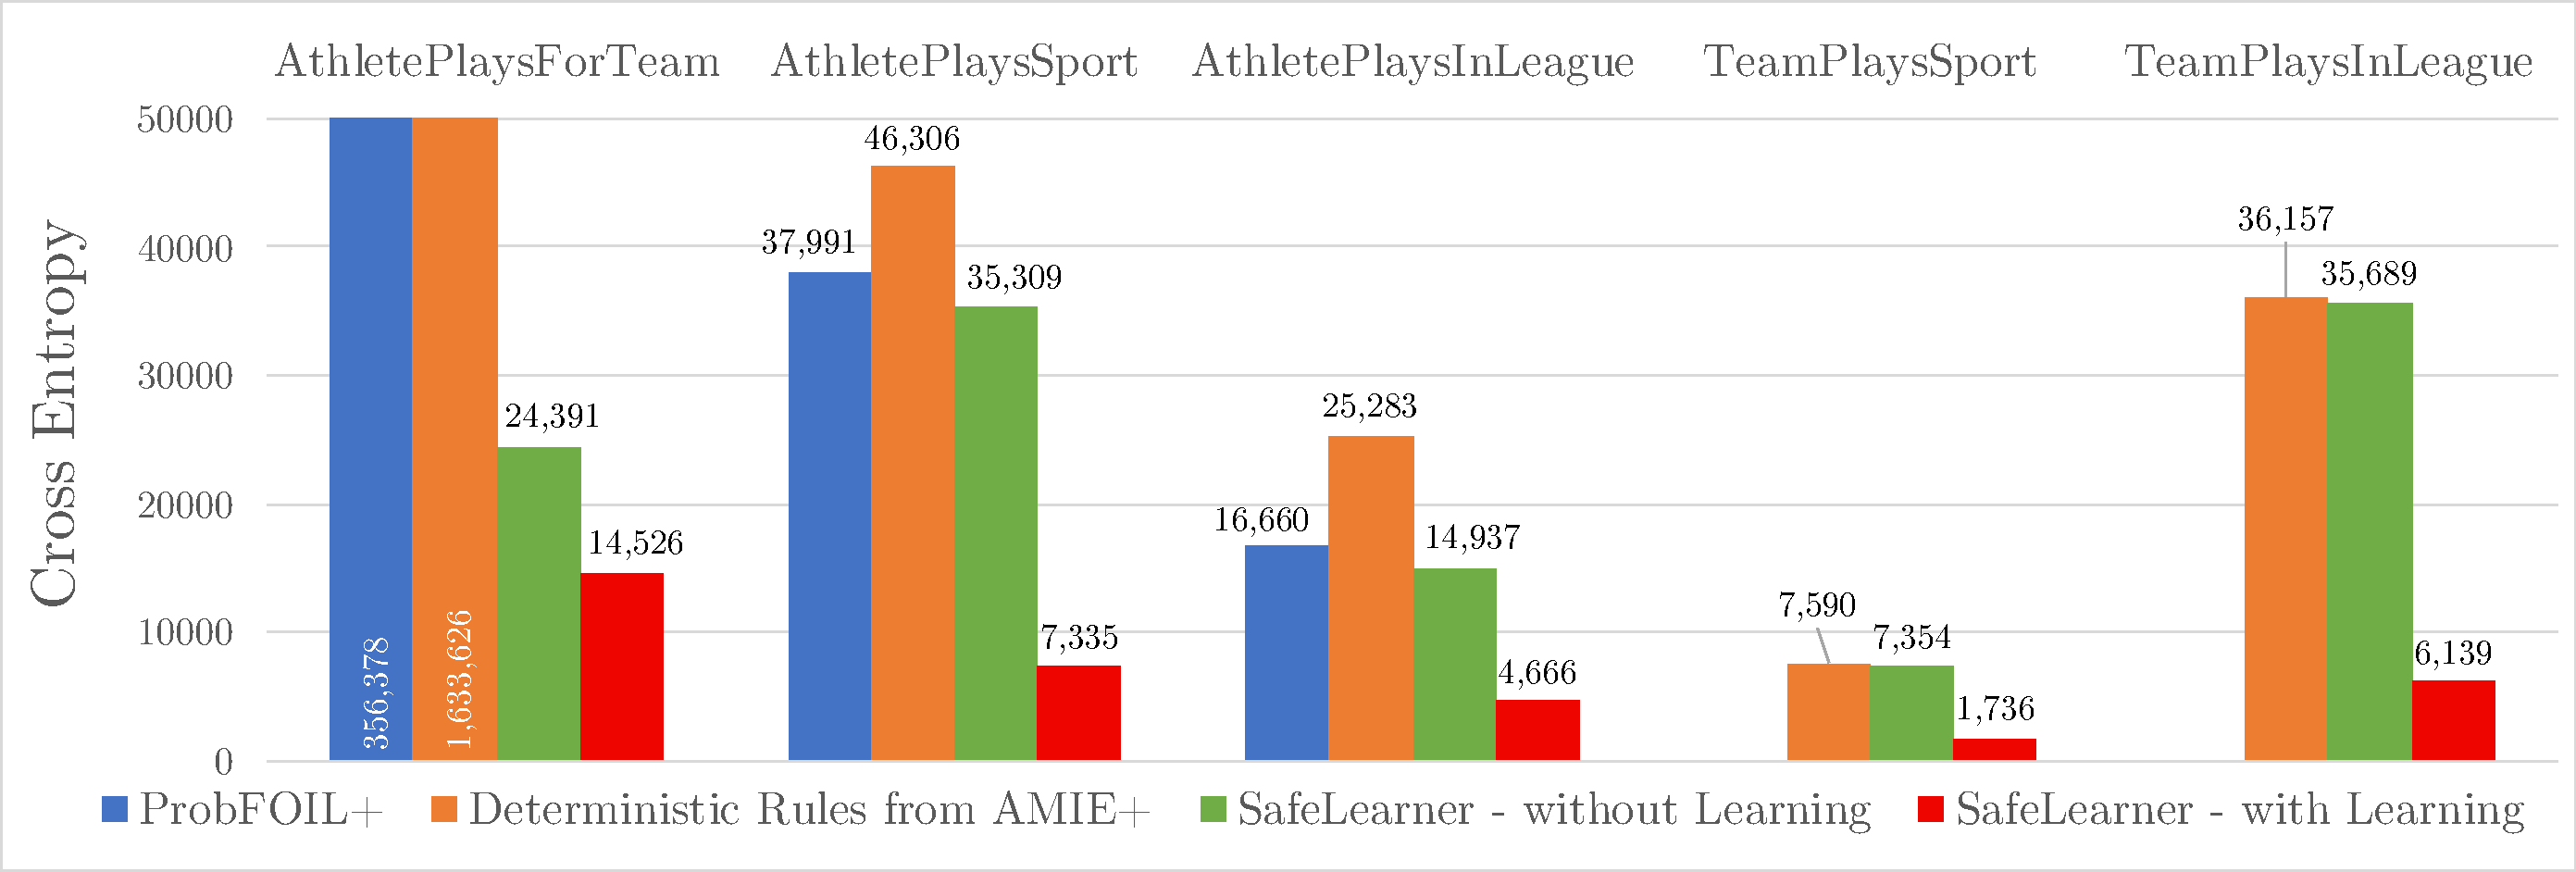
\includegraphics{WithNoiseCW/Exp1_CE_v4.pdf}}\caption{\algorithmname has better cross entropy than its baselines}\label{fig:CrossEntropy}\ \\
\end{center}
\end{figure}
\begin{figure}[h]
\begin{center}
    \begin{tabular}{@{}c@{}c@{}c@{}}
        \scalebox{.33}{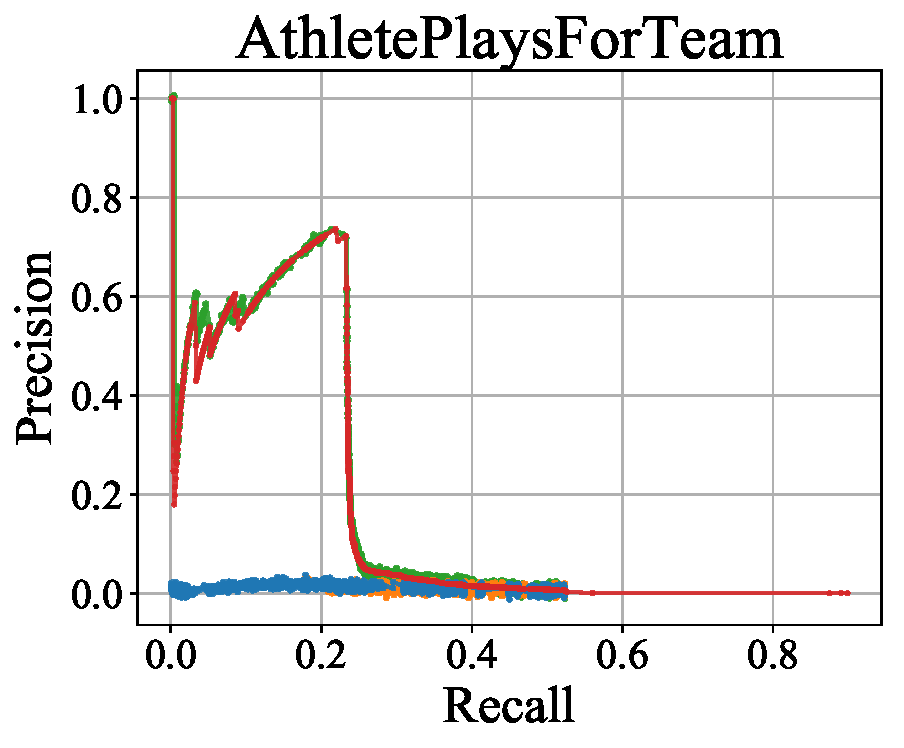
\includegraphics{WithNoiseCW/Exp1_apft_det.pdf}} & \scalebox{.33}{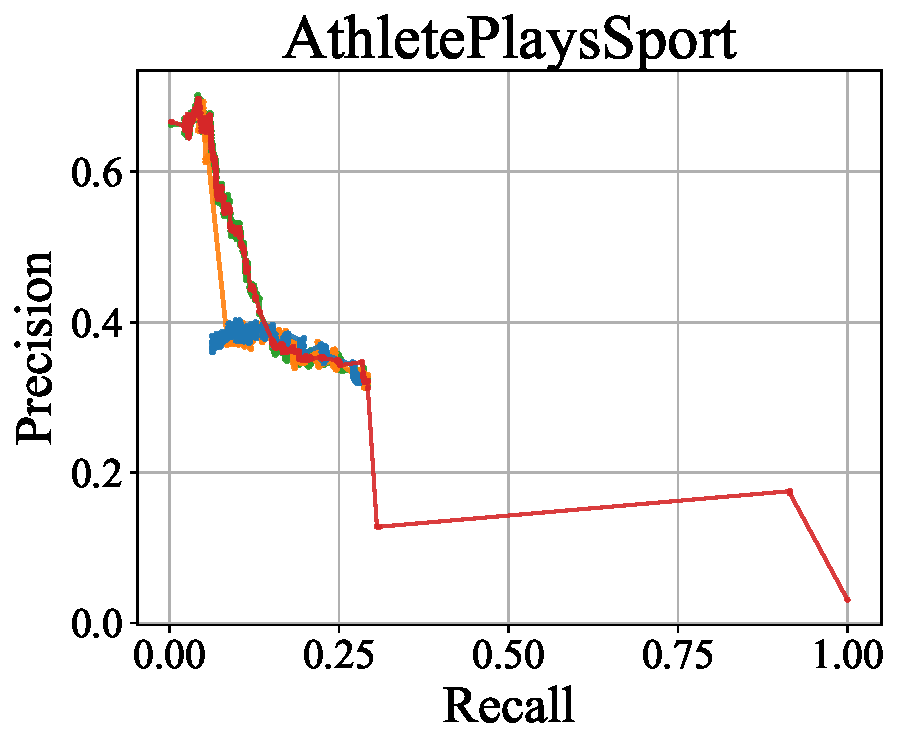
\includegraphics{WithNoiseCW/Exp1_aps_det.pdf}} & \scalebox{.33}{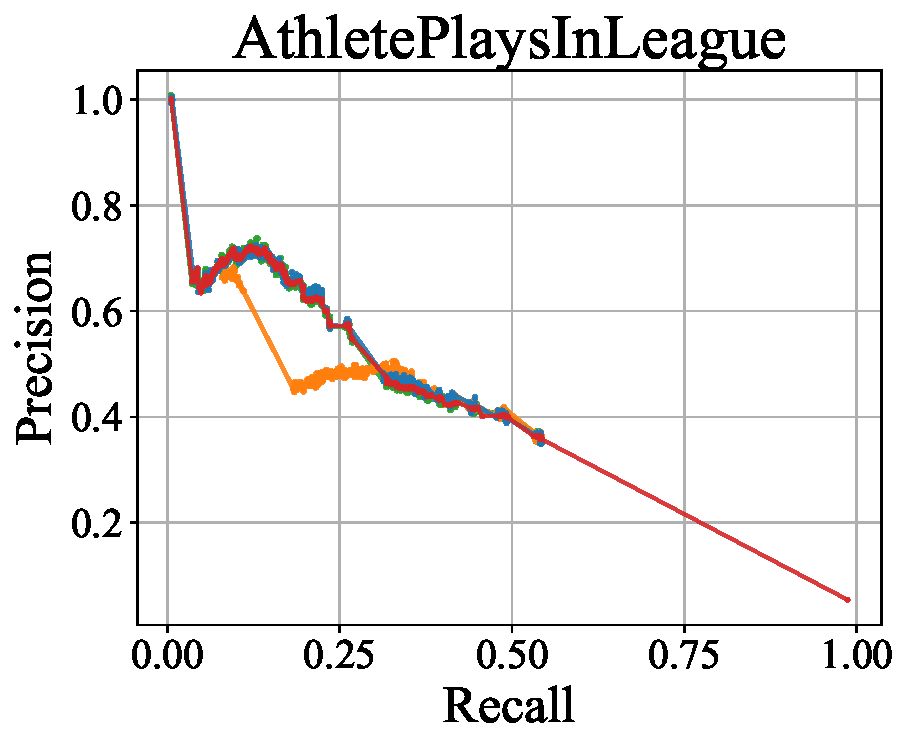
\includegraphics{WithNoiseCW/Exp1_apil_det.pdf}} \\
        \scalebox{0.8}{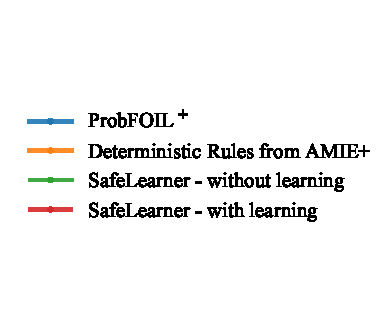
\includegraphics{WithNoiseCW/legend.pdf}} & \scalebox{.33}{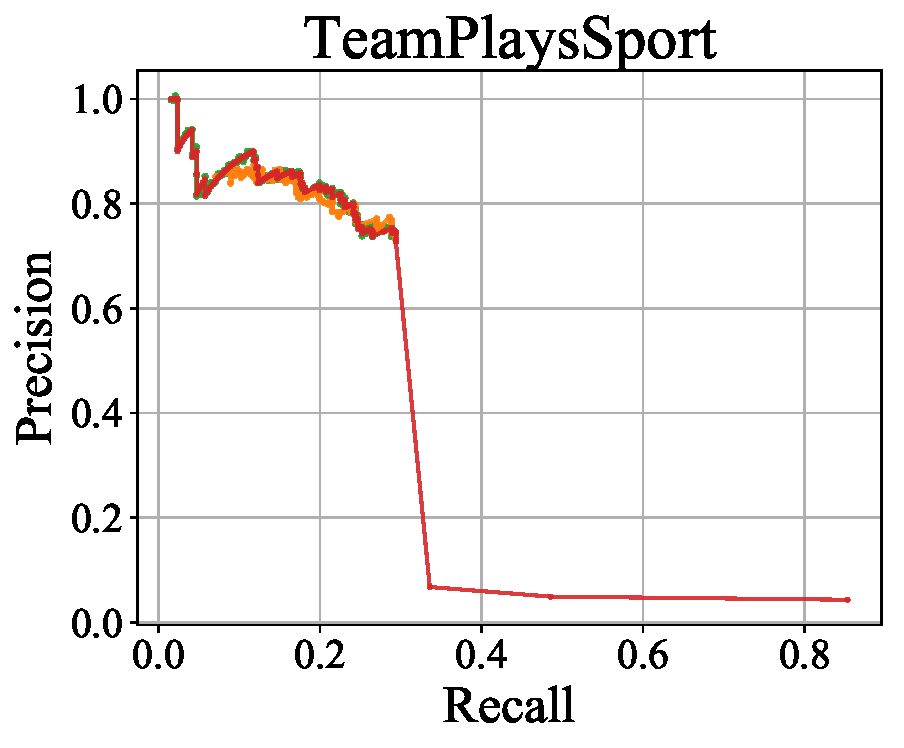
\includegraphics{WithNoiseCW/Exp1_tps_det.pdf}} & \scalebox{.33}{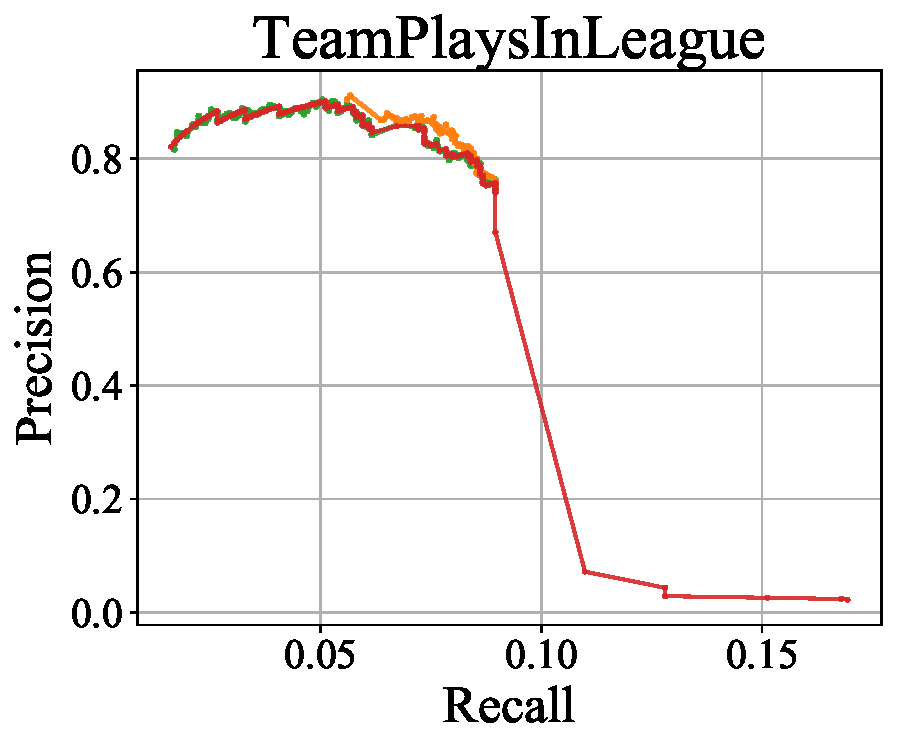
\includegraphics{WithNoiseCW/Exp1_tpil_det.pdf}}
    \end{tabular}\caption{Precision-Recall Curves for 5 relations in NELL Sports Dataset} \label{fig:PRCurves}%\guy{fonts are very small: split in two columns?}
\end{center}
\end{figure}

\subsection{How well does \algorithmname scale-up?}
\paragraph{Datasets:} 
This question attempts to test and stretch the limits of \algorithmname by measuring its scalability. We emperically show that \algorithmname scales on the latest iteration of full database of NELL (iteration:1115) with 233,000 tuples and 426 relations.  It can also scale up to the standard subset of Yago 2.4 \footnote{Yago is available at \url{http://yago-knowledge.org/}} with 948,000 tuples and 33 relations. (For Yago 2.4, the confidence in the collection of a relation was considered to be the probability of all the tuples of that relation.) \\

\begin{table}[H]
\centering
\begin{tabular}{|c|c|c|c|c|}
\hline
\multirow{2}{*}{KB} & \multirow{2}{*}{$target$ relation} & No. of $target$ & No. of rules & \multirow{2}{*}{Runtime}\\
 & & tuples & learned & \\
\hline
NELL & AthletePlaysForTeam	& \ 1687 & 3 & 1 hour \ 11 minutes \\
NELL & AthletePlaysSport	& \ 1959 & 5 & 2 hours \ 8 minutes \\
NELL & AthletePlaysInLeague & \ 1310 & 5 & 1 hour \ 34 minutes\\
NELL & TeamPlaysSport		& \ \ 355 & 5 & 5 hours 16 minutes \\
NELL & TeamPlaysInLeague	&\ 1354 & 5 & 3 hours \ 1 minute\ \ \\
YAGO & IsCitizenOf          &14554 & 4 & 2 hours 25 minutes \\
\hline
\end{tabular}
\caption{\algorithmname is able to scale-up to large scale KBs}\label{table:scaleup}
\end{table}

\paragraph{Results:} 
From Table \ref{table:scaleup}, it can be easily seen that although \algorithmname suffers in runtime when it learns more rules, it is able to scale to more than 14000 $target$ tuples (in case of Yago:IsCitizenOf) in relatively lesser time as it learns fewer rules. It would also depend upon how complex the learned rules are. The actual rules learned by \algorithmname are mentioned in the Appendix \ref{appendix:2}. To resolve this trade-off between runtime and number of rules, we could also specify the maximum number of rules to learn as part of the input parameters.

\section{Related Work and Discussion}
\label{sec:related}
The work presented in this paper advances the works \cite{DBLP:conf/ijcai/RaedtDTBV15,theobald_learning} that also studied learning in the probabilistic database setting.\footnote{Strictly speaking, the work \cite{DBLP:conf/ijcai/RaedtDTBV15} was framed within the probabilistic logic programming setting. However, probabilistic logic programming systems, such as Problog \cite{fierens2015inference}, can be seen as generalizations of probabilistic databases.} 
%The main differences with respect 
But compared with these previous works, we rely on lifted inference, which allows our approach to scale to much larger databases. %Second, we work in the open-world settings which allows us to model realistic datasets more faithfully because we do not have to assume that every tuple not present in the database is false. Third, 
Both of the previous approaches only use tuples from a given training set but do not take into account the behavior of the model on tuples not in the training set. 
This is problematic %\guy{some steps are missing in this discussion} 
because, unless the training set is really large, these previous methods do not distinguish models that predict too many false positives (i.e. models that give too high probability to too many tuples outside the training set). This becomes an issue especially in sparse domains (and most real domains are indeed sparse).

Our work is also closely related to the literature on learning from knowledge bases such as NELL within statistical relational learning (SRL), including works that use Markov logic networks \cite{DBLP:conf/emnlp/SchoenmackersDEW10}, Bayesian logic programs \cite{raghavan2012learning} and stochastic logic programs \cite{lao2011random,wang2014structure}. A disadvantage of many of these methods is that the learned parameters of the models can not be interpreted easily, which is particularly an issue for Markov logic networks where the weight of a rule cannot be understood in isolation from the rest of the rules. In contrast, the learned weights of probabilistic rules in our work, and also in the other works relying on probabilistic databases \cite{DBLP:conf/ijcai/RaedtDTBV15,theobald_learning}, have a clear probabilistic interpretation.

\paragraph{Parameter Learning with Different Losses}

Cross entropy is not the only loss function that may be considered for learning the parameters of probabilistic rules. Here, we discuss two additional loss functions that have already been used for the same or similar tasks in the literature: {\em squared loss} \cite{theobald_learning} and a probabilistic extension of accuracy \cite{DBLP:conf/ijcai/RaedtDTBV15}. Whereas cross entropy and squared loss belong among so-called {\em proper scoring rules} \cite{gneiting2007strictly} and, thus, reward estimates of probabilities that match the true probability, this is not the case for probabilistic accuracy. Moreover, each of these functions also relies on additional assumptions such as mutual independence of the examples' probabilities as well as mutual independence of the predictions, although this is not mentioned explicitly in the respective works \cite{theobald_learning,DBLP:conf/ijcai/RaedtDTBV15}. Below, we briefly discuss squared loss and probabilistic accuracy.

\paragraph{Squared Loss (Brier Score)}

As before, let $p_i$ denote the probability of the $i$-th example and $q_i$ the probability of the respective prediction. Then, the squared loss, which is a proper scoring rule, is:
$L_{sq} = \frac{1}{|E|}\sum_{\langle t_i, p_i \rangle \in E} p_i (1-q_i)^2 + (1-p_i) q_i^2.$
Minimizing $L_{sq}$ is also equivalent to minimizing the loss $L_{sq}' = \frac{1}{E} \sum_{\langle t_i, p_i \rangle \in E} \left(p_i - q_i \right)^2$
which was among others used in \cite{theobald_learning} for learning probabilities of tuples in PDBs.

\paragraph{Probabilistic Accuracy}

\citeauthor{DBLP:conf/ijcai/RaedtDTBV15} (\citeyear{DBLP:conf/ijcai/RaedtDTBV15}) define probabilistic extension of accuracy and other measures of predictive quality such as precision and recall. Their version of probabilistic accuracy is
$\textit{Acc}_{\textit{prob}} = 1-\frac{1}{|E|} \sum_{\langle t_i, p_i \rangle \in E} \left| p_i - q_i \right|.$
Unlike the other two discussed loss functions, probabilistic accuracy is not a proper scoring rule as the next example illustrates, however, it has other convenient properties (cf. \citet{DBLP:conf/ijcai/RaedtDTBV15} for details). 
\begin{example}
Let the set of domain elements in the database be $\mathcal{C} = \{\mathsf{alice}, \mathsf{bob}, \mathsf{eve} \}$. Next, let $E = \{ \langle [\mathsf{alice}], 0 \rangle, \langle [\mathsf{bob}], 1 \rangle, \langle [\mathsf{eve}], 1 \rangle \}$ be the set of training examples for the relation $\mathsf{smokes}$ and let us have the rule $p :: \mathsf{smokes}(X) \mbox{ \textnormal{:--}}\; \mathsf{true}$. Then, maximizing probabilistic accuracy on $E$ yields $p = 1$, whereas optimizing both cross entropy and squared loss would yield $p = 2/3$, which is the probability that a randomly selected person in $\mathcal{C}$ smokes.
\end{example}

\section{Conclusions}
\label{sec:conc}
We proposed a probabilistic rule learning system, named \algorithmname, that supports lifted inference. It first performs structure learning by mining independent deterministic candidate rules using AMIE+ and later executes joint parameter learning over all the rule probabilities.
% and the open-world parameters for all the relations.
\algorithmname extends ProbFOIL$^+$ by using lifted probabilistic inference (instead of using grounding). 
%Firstly, it follows Open-World Assumption (OWA) (instead of CWA) and secondly, it uses lifted probabilistic inference (instead of grounding). 
Therefore, it scales better than ProbFOIL$^+$. In comparison with AMIE+, it is able to jointly learn probabilistic rules over a probabilistic KB unlike AMIE+ which only learns independent deterministic rules (with confidences) over a deterministic KB. We experimentally show that \algorithmname scales as good as AMIE+ when learning simple rules. Trying to learn complex rules leads to unsafe queries which are not suitable for lifted inference. But lifted inference helps \algorithmname in outperforming ProbFOIL$^+$ which does not scale to NELL Sports Database without the help of a declarative bias. 
%Our experiments also exhibit that the OWA does not significantly improve the quality of rules. This is because most of the KBs in real-world are highly sparse and incomplete. Although, \algorithmname could also be run under CWA for faster results on large KBs, OWA still remains to be further tested on more diverse probabilistic KBs.

A few limitations of \algorithmname are described as follows. Firstly, it cannot learn complex rules that translate to an unsafe query. Secondly, it does not use rules within the background theory. %Thirdly, although it is open-world, it is not open-universe. This is because \algorithmname assumes that all the constants of all the types of entities are known. 
Lastly, it can not learn rules on $PDB$ with numeric fields (without assuming them as discrete constants).

The main contributions of \algorithmname are presented as follows. Firstly, it accomplishes probabilistic rule learning using a novel inference setting as it is the first approach that uses lifted inference for KB completion. Secondly, unlike ProbFOIL$^+$, \algorithmname scales well on the full database of NELL with 233,000 tuples and 426 relations as well as on the standard subset of Yago 2.4 with 948,000 tuples and 33 relations. Thirdly, \algorithmname is faster than ProbFOIL$^+$ because of the following three factors: 1) it disintegrates longer complex queries to smaller simpler ones, 2) it caches the structure of queries before doing inference and 3) it uses lifted inference to infer on those simple queries. The first two factors of query disintegration and memoization are discussed in Appendix \ref{appendix:4} in further detail.

In future, this work could be advanced further to eliminate its shortcomings. In particular, a prominent direction of advancement would be to extend probabilistic rule learning to open-world setting of which the $Lift^O_R$ algorithm \cite{DBLP:conf/kr/CeylanDB16} is capable.

\section*{Acknowledgements}
The authors express their sincere regards to Anton Dries and Sebastijan Duman\u{c}i\'c for their invaluable input, and the reviewers for their useful suggestions. This work has received funding from the European Research Council (ERC) under the European Union’s Horizon 2020 research and innovation programme (grant agreement no [694980] SYNTH: Synthesising Inductive Data Models).

\bibliographystyle{plainnat}
\bibliography{Bibliography}

\appendix
\section{NELL Sports Dataset at 850$^{\mbox{\tiny th}}$ iteration}\label{appendix:1}

\begin{table}[H]
\centering
\begin{tabular}{ll|c}
Relations			&Types				& No. of tuples\\
\hline
athleteledsportsteam&(athlete,team) 	& 246\\
athleteplaysforteam	&(athlete,team)		& 808\\
athleteplaysinleague&(athlete,league) 	& 1197\\
athleteplayssport	&(athlete,sport) 	& 1899\\
teamalsoknownas	    &(team,team) 		& 273\\
teamplaysagainstteam&(team,team) 		& 2848\\
teamplaysinleague	&(team,league) 		& 1229\\
teamplayssport		&(team,sport) 		& 340\\
\end{tabular}
\caption{Relations present in NELL Sports Dataset at 850$^{\mbox{\tiny th}}$ iteration}\label{table:nell}
\end{table}

\section{Rules learned in Experiment 2}\label{appendix:2}

%\arcchit{Checked for True Rules}\\
\begin{footnotesize}
\begin{tabular}{|l|}
\hline
\textbf{NELL:AthletePlaysForTeam} \\
0.118863::athleteplaysforteam(A,B) :- athleteledsportsteam(C,B), teammate(A,C) \\
0.118863::athleteplaysforteam(A,B) :- athleteledsportsteam(C,B), teammate(C,A) \\
0.005193::athleteplaysforteam(A,B) :- athleteplayssport(A,C), teamplayssport(B,C) \\[2ex]
%Number of $\mathsf{AthletePlaysForTeam}$ tuples = 1687 \\
%Learning Time = 1 hour 11 minutes \\ %4306 seconds      
%\hline
\textbf{NELL:AthletePlaysSport} \\
0.408582::athleteplayssport(A,B) :- athleteledsportsteam(A,C), teamplayssport(C,B) \\
0.329230::athleteplayssport(A,B) :- athleteplaysforteam(A,C), teamplayssport(C,B) \\
0.236742::athleteplayssport(A,B) :- athletehomestadium(A,C), stadiumhometosport(C,B) \\
0.051982::athleteplayssport(A,B) :- athleteplayssportsteamposition(A,C), sportsteampositionforsport(C,B) \\
0.012186::athleteplayssport(A,B) :- athleteflyouttosportsteamposition(A,C), sportsteampositionforsport(C,B) \\[2ex]
%Number of $\mathsf{AthletePlaysSport}$ tuples = 1959 \\
%Learning Time = 2 hours 8 minutes \\ %7708 seconds
%\hline
\textbf{NELL:AthletePlaysInLeague} \\
0.02987::athleteplaysinleague(A,B) :- true \\
0.78947::athleteplaysinleague(A,B) :- athletecoach(A,C), coachesinleague(C,B) \\
0.51818::athleteplaysinleague(A,B) :- athleteledsportsteam(A,C), teamplaysinleague(C,B) \\
0.33935::athleteplaysinleague(A,B) :- athleteplaysforteam(A,C), teamplaysinleague(C,B) \\
0.33560::athleteplaysinleague(A,B) :- athletehomestadium(A,C), stadiumhometoleague(C,B) \\[2ex]
%Number of $\mathsf{AthletePlaysInLeague}$ tuples = 1310 \\
%Learning Time = 1 hours 34 minutes \\ %5687 seconds
%\hline
\textbf{NELL:TeamPlaysSport}  \\
0.10014::teamplaysinleague(A,B) :- true \\
0.74590::teamplaysinleague(A,B) :- athleteledsportsteam(C,A), athleteplaysinleague(C,B) \\
0.72185::teamplaysinleague(A,B) :- stadiumhometoleague(C,B), teamhomestadium(A,C) \\
0.68::teamplaysinleague(A,B) :- athleteplaysforteam(C,A), athleteplaysinleague(C,B) \\
0.57576::teamplaysinleague(A,B) :- coachesinleague(C,B), coachesteam(C,A) \\[2ex]
%Number of $\mathsf{TeamPlaysSport}$ tuples = 355 \\
%Learning Time = 5 hours 16 minutes \\ %18936 seconds
%\hline
\textbf{NELL:TeamPlaysInLeague} \\
0.10014::teamplaysinleague(A,B) :- true \\
0.74590::teamplaysinleague(A,B) :- athleteledsportsteam(C,A), athleteplaysinleague(C,B) \\
0.72185::teamplaysinleague(A,B) :- stadiumhometoleague(C,B), teamhomestadium(A,C) \\
0.68::teamplaysinleague(A,B) :- athleteplaysforteam(C,A), athleteplaysinleague(C,B) \\
0.57575::teamplaysinleague(A,B) :- coachesinleague(C,B), coachesteam(C,A) \\[2ex]
%Number of $\mathsf{TeamPlaysInLeague}$ tuples = 1354 \\
%Learning Time = 3 hours 1 minute \\ %10854 seconds
%\hline
\textbf{YAGO:IsCitizenOf} \\
0.00651::iscitizenof(A,B) :- true \\
0.2::iscitizenof(A,B) :- hascapital(B,C), holdspoliticalposition(A,C) \\
0.10435::iscitizenof(A,B) :- hasacademicadvisor(C,A), livesin(C,B) \\
0.1::iscitizenof(A,B) :- livesin(A,C), participatedin(B,C) \\
%Number of $\mathsf{IsCitizenOf}$ tuples = 14554 \\
%Learning Time = 2 hours 25 minutes \\ %8708 seconds
\hline
\end{tabular}\\
\end{footnotesize}


\section{How well does ProbFOIL$^+$ scale-up in comparison to \algorithmname?}\label{appendix:3}
To answer this question, we generated 13 probabilistic knowledge bases with different number of tuples ranging from 10 to 100k. To generate a KB of size $n$, uniform random probability values were assigned to $n$ different tuples of the $target$ relation $a$ and these values were scaled down by an arbitrary constant factor of 0.18 and assigned to $n$ other tuples of a non-target relation $b$. 

\begin{figure}[H]
\begin{center}
    \scalebox{0.425}{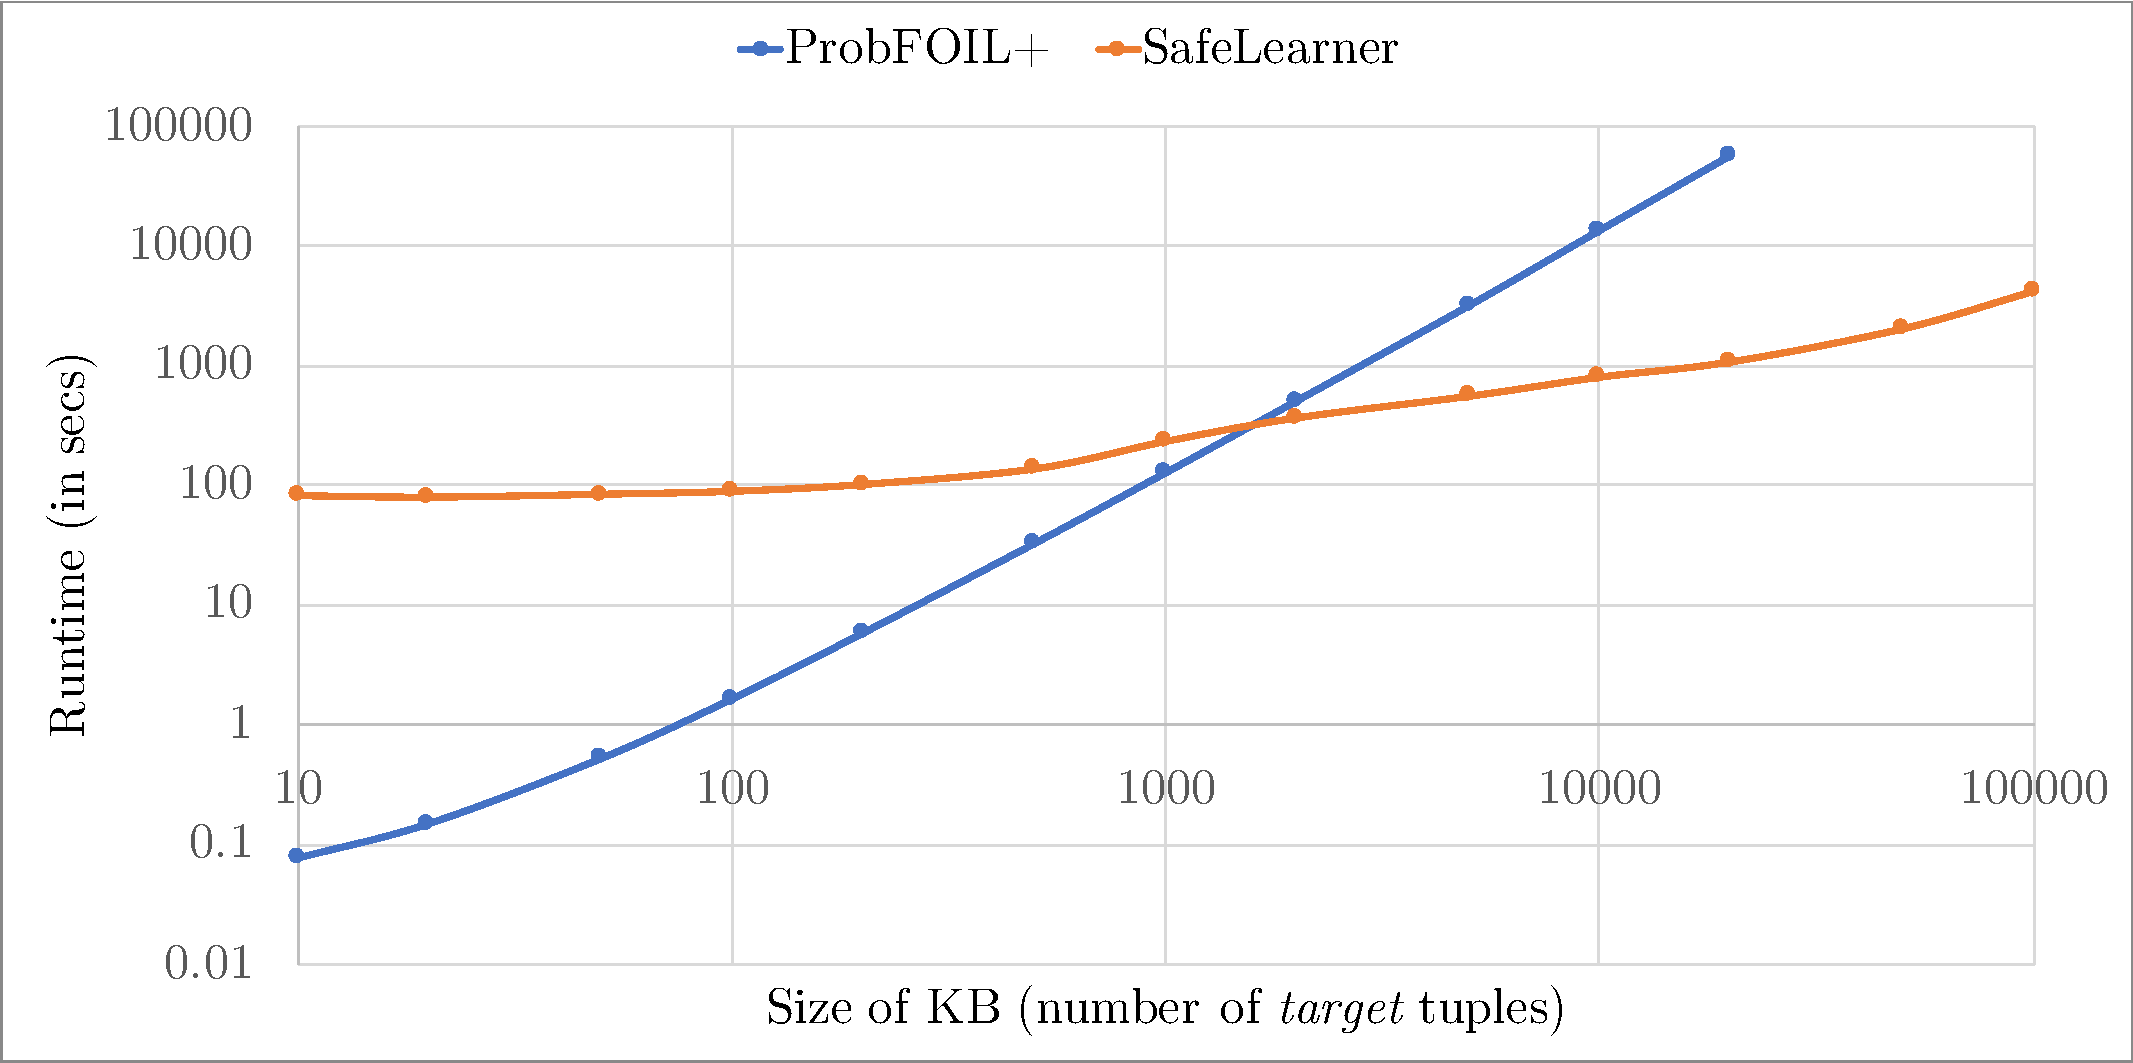
\includegraphics{Rebuttal/ScalingExperiment3.pdf}}\caption{\algorithmname is much faster than ProbFOIL$^+$ in large scale Probabilistic KBs}\label{fig:scaleup}
\end{center}
\end{figure}

As seen clearly from the Figure \ref{fig:scaleup}, ProbFOIL$^+$ struggles to scale upto large KBs with number of $target$ tuples $> 5000$. On the other hand, such large KBs are handled much faster by \algorithmname. For instance, for a simple probabilistic KB with 20000 $target$ tuples and 20000 non-target tuples, ProbFOIL$^+$ took 15 hours and 54 minutes and \algorithmname took just 30 minutes. 

%\arcchit{Explain why are there only 2 relations in artificial KBs} 
This experiment may seem frail at first glance as it uses artificially created datasets. But this is done only to make ProbFOIL$^+$ faster as it would lead to only 4 candidate rules: $\mathsf{a}$($X, Y$) :- $\mathsf{true}$., $\mathsf{a}$($X, Y$) :- $\mathsf{fail}$., $\mathsf{a}$($X, Y$) :- $\mathsf{b}$($X, Y$)., and $\mathsf{a}$($X, Y$) :- $\mathsf{b}$($Y, X$).\ . The number of candidate rules are minimized in purpose to demonstrate that the lag in ProbFOIL$^+$ occurs due to the size of the KB instead of the number of candidate rules it has to consider while learning.

\section{How much does different components of \algorithmname boost its runtime?}\label{appendix:4}

As mentioned in the section \ref{sec:conc}, apart from lifted inference, \algorithmname gets speed-up due to memoization/caching and disintegration of longer complex queries before calling SlimShot.

\paragraph{Memoization}
\algorithmname uses memoization before calling SlimShot in order to minimize runtime by storing the results of the expensive function call to SlimShot and returning the cached result when the structure of the query occurs again in the input. Since SlimShot produces a query plan, we exploit the fact that isomorphic queries naturally have the same query plans. For example, since both queries $Q_1 = \mathsf{a}(X,Y),\mathsf{b}(Y)$ and $Q_2 = \mathsf{x}(A,B), \mathsf{y}(B)$ have the same canonical structure $\mathsf{table1}(Var1, Var2), \mathsf{table2}(Var2)$, they have the same sequence of SQL operations to calculate their probabilities. Thus, using memoization, we eliminate the need to call SlimShot for $Q_2$ if we have already called it befor for $Q_1$. 

\paragraph{Query Disintegration} 
The query disintegration step is introduced in Algorithm \ref{alg:predictProb} in Section \ref{sec:algo}. In ProbabilityPredictor, the input query $Q = q_1 \vee q_2 \vee \cdots q_n$ is first broken down in line \ref{alg_line:disjunctList} to a list of each of the separate disjuncts ([$q_1, q_2, \ldots , q_n$]). Now since each disjunct can be written as a conjunction of relations from in the KB, line \ref{alg_line:mergeDisjuncts} merges all those disjuncts together that share at least one relation. Each element in $disjunctList$ can now be thought of as a separate sub-query which does not share any relations with any other sub-query. The following loop calculated the probability of each of the subqueries and then unifies the probability in line \ref{alg_line:unifyProbs}.

Theoretically, if $Q$ can be written as a union of independent subqueries, i.e., 
$Q = s_1 \vee s_2 \vee \cdots s_m$ where $s_i$, $s_j$ don't share any relation for all $i, j$ in $\{1, 2, \ldots, m\}$, $m \leq n$, then\\
\begin{equation}
    \mathrm{P}(Q) = 1 - \prod_{i = 1}^m(1 - \mathrm{P}(s_i))
\end{equation}

%\arcchit{Argue about why is it different from the one whihc is handled inside SlimShot}
One could argue that there is no need to do query disintegration step outside SlimShot as it happens inside it within its lifted inference engine. But as SlimShot does not do memoization internally, it may end up finding query plans for isomorphic subqueries. And in \algorithmname, this may happen frequently if a lot of candidate rules are isomorphic and independent to one another. Thus, introducing the query disintegration would complement memoization step in the above mentioned case.

\paragraph{Result}
We ran 4 versions of \algorithmname to emperically evaluate the extent of the speed-up we get form these two techniques. We compared these versions on NELL(iteration:850) for $target$ = $\mathsf{AthletePlaysForTeam}$ as well as on YAGO for $target$ = $\mathsf{IsCitizenOf}$. Although there is significant speed-up when both the techniques are present as compared to when these are absent, it is interesting to note that the runtime of Version 3 for NELL is better than that of Version 1. This happened because the learned rules were not complicated enough and not trying to disintegrate simpler queries resulted in a slightly faster performance.

\begin{table}[H]
\centering
\begin{tabular}{|c|c|c|c|c|}
\hline
\multirow{2}{*}{Version No.}	& \multirow{2}{*}{Memoization}	 & \multirow{2}{*}{Query Disintegation} &	 \multicolumn{2}{c|}{Runtime (in secs)}\\
\cline{4-5}
& & & NELL & YAGO \\
\hline
1 & $\checkmark$ & $\checkmark$ & \ 4183 & 20398\\
2 & $\times$ & $\checkmark$ & 13490 & 27246\\
3 & $\checkmark$ & $\times$ & \ 4125 & 20503\\
4 & $\times$ & $\times$ & 16461 & 30535\\
\hline
\end{tabular}
\caption{Memoization and Query Disintegration speed-up by 50\% and 7\% respectively}\label{table:speedup}
\end{table}

\section{For KB completion, how does the Statistical Relational Learning (SRL) based approach of \algorithmname compare against Knowledge Graph Embeddings (KGE) based approaches?}\label{appendix:5}

%General comments about the difference in approaches
We have compared the SRL based approach with the KGE based approach for KB completion over the following 4 criteria:
\begin{enumerate}
    \item \textbf{Interpretability and explainability:} \algorithmname uses Statistical Relational Logic (SRL) based approach to do KB completion which allows it to infer new tuples based on learned rules. This makes the SRL based approach interpretable and explainable as compared to the black-box KGE based approaches.
    \item \textbf{Scalability:} Traditionally KGE based approaches were considered to be more scalable than the SRL based approaches but this is not the case now. \algorithmname, an SRL based approach, has shown that it could scale to large scale KBs (YAGO with 948,000 tuples and NELL with 233,000 tuples) as it is the first approach to use lifted inference. This is at least at par with the scale of KBs handled in KGE based approaches.
    \item \textbf{Sparsity and Reasoning:} Since an SRL based approach would learn first-order rules to predict tuples, it can even reason about new constants being included in the KB without re-training. A KGE based approach may discard the existence of a tuple with a new constant as the embedding for the new constant does not exist. Thus it is easier for SRL based approaches to handle highly sparse KBs as they can handle the high number of constants since they only learn first order rules. A KGE based approach on a highly sparse KB would have to create a very large KGE due to high number of constants. And since the memory of GPUs is limited, KGE based approaches often have a practical restriction on the number of constants (to the order of 50k constants) they could handle. This limitation on the number of constants in a KB is not there when SRL based approaches are used.
    \item \textbf{Versatility:} SRL based approaches like \algorithmname treat probabilities in a principled manner while reasoning. On the other hand, in order to handle uncertainty in KBs, KGE based approaches return a confidence number but not a probability. And if the confidence scores are not well calibrated, then these can not be used as a proxy for probabilities. Thus KGE based approaches are more suitable in dealing with deterministic KBs. But SRL based approaches can deal with probabilistic KBs as well as deterministic KBs making them more versatile than KGE based approaches for KB completion.
\end{enumerate}

%\arcchit{Please help in adding more citations here to second our arguments.}\\
As concluded by \citet{DBLP:journals/corr/abs-1806-11391}, apart from the limited reasoning capabilities and black-box nature, another major disadvantage of KGEs is their sensitivity to hyper-parameters. But there are few advantages of using KGE based approaches. These approaches are more suitable to a curated data and can exploit the similarity structure encoded in KGEs. That is why, a futuristic and ideal approach for KB completion would be to combine the simple relational reasoning from KGE based approaches with the complex reasoning from SRL based approaches.

%\arcchit{Eventually one should combine the 2 approaches and it could be a future step}


\end{document}